\documentclass{article}
\usepackage{fullpage}
\usepackage[utf8]{inputenc}
\usepackage{pict2e}
\usepackage{amsmath}
\usepackage{enumitem}
\usepackage{eurosym}
\usepackage{mathtools}
\usepackage{amssymb, amsfonts, latexsym, cancel}
\setlength{\parskip}{0.3cm}
\usepackage{graphicx}
\usepackage{fontenc}
\usepackage{slashbox}
\usepackage{setspace}
\usepackage{gensymb}
\usepackage{accents}
\usepackage{adjustbox}
\setstretch{1.35}
\usepackage{bold-extra}
\usepackage[document]{ragged2e}
\usepackage{subcaption}
\usepackage{tcolorbox}
\usepackage{xcolor, colortbl}
\usepackage{wrapfig}
\usepackage{empheq}
\usepackage{array}
\usepackage{parskip}
\usepackage{arydshln}
\graphicspath{ {images/} }
\renewcommand*\contentsname{\color{black}Índice} 
\usepackage{array, multirow, multicol}
\definecolor{lightblue}{HTML}{007AFF}
\usepackage{color}
\usepackage{etoolbox}
\usepackage{listings}
\usepackage{mdframed}
\setlength{\parindent}{0pt}
\usepackage{underscore}
\usepackage{hyperref}
\usepackage{tikz}
\usepackage{tikz-cd}
\usetikzlibrary{shapes, positioning, patterns}
\usepackage{tikz-qtree}
\usepackage{biblatex}
\usepackage{pdfpages}
\usepackage{pgfplots}
\usepackage{pgfkeys}
\addbibresource{biblatex-examples.bib}
\usepackage[a4paper, left=1cm, right=1cm, top=1cm,
bottom=1.5cm]{geometry}
\usepackage{titlesec}
\usepackage{titletoc}
\usepackage{tikz-3dplot}
\usepackage{kbordermatrix}
\usetikzlibrary{decorations.pathreplacing}
\newcommand{\Ej}{\textcolor{lightblue}{\underline{Ejemplo}}}
\setlength{\fboxrule}{1.5pt}

% Configura el formato de las secciones utilizando titlesec
\titleformat{\section}
{\color{red}\normalfont\LARGE\bfseries}
{Tema \thesection:}
{10 pt}
{}

% Ajusta el formato de las entradas de la tabla de contenidos
\addtocontents{toc}{\protect\setcounter{tocdepth}{4}}
\addtocontents{toc}{\color{black}}

\titleformat{\subsection}
{\normalfont\Large\bfseries\color{red}}{\thesubsection)}{1em}{\color{lightblue}}

\titleformat{\subsubsection}
{\normalfont\large\bfseries\color{red}}{\thesubsubsection)}{1em}{\color{lightblue}}

\newcommand{\bboxed}[1]{\fcolorbox{lightblue}{lightblue!10}{$#1$}}
\newcommand{\rboxed}[1]{\fcolorbox{red}{red!10}{$#1$}}

\DeclareMathOperator{\N}{\mathbb{N}}
\DeclareMathOperator{\Z}{\mathbb{Z}}
\DeclareMathOperator{\R}{\mathbb{R}}
\DeclareMathOperator{\Q}{\mathbb{Q}}
\DeclareMathOperator{\K}{\mathbb{K}}
\DeclareMathOperator{\im}{\imath}
\DeclareMathOperator{\jm}{\jmath}
\DeclareMathOperator{\col}{\mathrm{Col}}
\DeclareMathOperator{\fil}{\mathrm{Fil}}
\DeclareMathOperator{\rg}{\mathrm{rg}}
\DeclareMathOperator{\nuc}{\mathrm{nuc}}
\DeclareMathOperator{\dimf}{\mathrm{dimFil}}
\DeclareMathOperator{\dimc}{\mathrm{dimCol}}
\DeclareMathOperator{\dimn}{\mathrm{dimnuc}}
\DeclareMathOperator{\dimr}{\mathrm{dimrg}}
\DeclareMathOperator{\dom}{\mathrm{Dom}}
\DeclareMathOperator{\infi}{\int_{-\infty}^{+\infty}}
\newcommand{\dint}[2]{\int_{#1}^{#2}}

\newcommand{\bu}[1]{\textcolor{lightblue}{\underline{#1}}}
\newcommand{\lb}[1]{\textcolor{lightblue}{#1}}
\newcommand{\db}[1]{\textcolor{blue}{#1}}
\newcommand{\rc}[1]{\textcolor{red}{#1}}
\newcommand{\tr}{^\intercal}

\renewcommand{\CancelColor}{\color{lightblue}}

\newcommand{\dx}{\:\mathrm{d}x}
\newcommand{\dt}{\:\mathrm{d}t}
\newcommand{\dy}{\:\mathrm{d}y}
\newcommand{\dz}{\:\mathrm{d}z}
\newcommand{\dth}{\:\mathrm{d}\theta}
\newcommand{\dr}{\:\mathrm{d}\rho}
\newcommand{\du}{\:\mathrm{d}u}
\newcommand{\dv}{\:\mathrm{d}v}
\newcommand{\tozero}[1]{\cancelto{0}{#1}}
\newcommand{\lbb}[2]{\textcolor{lightblue}{\underbracket[1pt]{\textcolor{black}{#1}}_{#2}}}
\newcommand{\dbb}[2]{\textcolor{blue}{\underbracket[1pt]{\textcolor{black}{#1}}_{#2}}}
\newcommand{\rub}[2]{\textcolor{red}{\underbracket[1pt]{\textcolor{black}{#1}}_{#2}}}

\author{Francisco Javier Mercader Martínez}
\date{}
\title{Señales y Sistemas\\Problemas Tema 1: Conceptos Básicos de Señales y Sistemas}

\begin{document}
\maketitle
\begin{enumerate}[label=\color{red}\textbf{\arabic*)}]
  \item \lb{Exprese cada uno de los siguientes números complejos en su parte real e imaginaria $(a+jb)$:}
    \begin{multicols}{2}
    \begin{itemize}[label=\color{red}\textbullet, leftmargin=*]
      \item $\lb{\dfrac{1}{2}e^{j\pi} =}\dfrac{1}{2}(\cos(\pi)+j\sin(\pi))=-\dfrac{1}{2}$
      \item $\lb{\dfrac{1}{2}e^{-j\pi} =}\dfrac{1}{2}(\cos(\pi)-j\sin(\pi))=-\dfrac{1}{2}$ 
      \item $\lb{e^{j\frac{\pi}{2} }=} \cos\left( \dfrac{\pi}{2} \right) +j\cdot \sin\left( \dfrac{\pi}{2} \right) =j$ 
      \item $\lb{e^{-j\frac{\pi}{2} } =} \cos\left( \dfrac{\pi}{2} \right) -j\cdot \sin\left( \dfrac{\pi}{2} \right) =-j$ 
      \item $\lb{e^{j\frac{5\pi}{2} } =} \cos\left( \dfrac{5\pi}{2} \right) +j\cdot \sin\left( \dfrac{5\pi}{2} \right) =j$ 
      \item $\lb{\sqrt{2} e^{j\frac{\pi}{4} } =}\sqrt{2}\cdot \left(\cos\left( \dfrac{\pi}{4} \right) +j\cdot \sin\left( \dfrac{\pi}{4} \right)\right) =1+j$ 
      \item $\lb{\sqrt{2} e^{j\frac{9\pi}{4} } =} \sqrt{2}\cdot  \left(\cos\left( \dfrac{9\pi}{4} \right) +j\cdot \sin\left( \dfrac{9\pi}{4} \right) \right)=1+j$ 
      \item $\lb{\sqrt{2} e^{-j\frac{9\pi}{4} } =} \sqrt{2}\cdot  \left(\cos\left( \dfrac{9\pi}{4} \right) -j\cdot \sin\left( \dfrac{9\pi}{4} \right)\right) =1-j$ 
      \item $\lb{\sqrt{2} e^{-j\frac{\pi}{4} } =} \sqrt{2}\cdot  \left(\cos\left( \dfrac{\pi}{4} \right) -j\cdot \sin\left( \dfrac{\pi}{4} \right)\right) =1-j$
    \end{itemize}
  \end{multicols}
  \item \lb{Exprese cada uno de los siguientes números complejos en su módulo y fase ($|z|e^{j\varphi(z)}$ con $\varphi(z)\in [-\pi,\pi]$):} 
      \begin{itemize}[label=\color{red}\textbullet, leftmargin=*]
        \item $\lb{5:}\begin{cases}
          |z|=\sqrt{5^2+0^2} =5\\
          \varphi=\arctan\left( \dfrac{0}{5} \right) =0
        \end{cases}\longrightarrow 5 $ 
        \item $\lb{-2:}\begin{cases}
          |z|=\sqrt{(-2)^2+0^2}=2\\
          \varphi=\arctan\left( \dfrac{0}{-2} \right) =\pi
        \end{cases} \longrightarrow 2e^{j\pi} $ 
        \item $\lb{-3j:} \begin{cases}
          |z|=\sqrt{0^2+(-3)^2}=3\\
          \varphi=\arctan\left( \dfrac{-3}{0} \right) =-\dfrac{\pi}{2}
        \end{cases}\longrightarrow 3e^{-j\frac{\pi}{2} } $ 
        \item $\lb{-j \dfrac{\sqrt{3} }{2}:} \begin{cases}
          |z|=\sqrt{0^2+\left( -\dfrac{\sqrt{3} }{2} \right) ^2}=\dfrac{\sqrt{3} }{2}\\
          \varphi=\arctan\left( \dfrac{-\frac{\sqrt{3} }{2} }{0} \right) =-\dfrac{\pi}{2}
        \end{cases}\longrightarrow \dfrac{\sqrt{3} }{2}e^{-j\frac{\pi}{2} } $ 
        \item $\lb{1+j:} \begin{cases}
          |z|=\sqrt{1^2+1^2}=\sqrt{2}\\
          \varphi=\arctan\left( \dfrac{1}{1} \right) =\dfrac{\pi}{4}
        \end{cases}\longrightarrow \sqrt{2}e^{j\frac{\pi}{4} }  $ 
        \item $\lb{(1-j)^2=-2j:} \begin{cases}
          |z|=\sqrt{0^2+(-2)^2}=2\\
          \varphi=\arctan\left( \dfrac{-2}{0} \right) =-\dfrac{\pi}{2}
        \end{cases}\longrightarrow 2e^{-j\frac{\pi}{2} } $ 
      \item $\lb{j(1-j)=1+j:} \begin{cases}
              |z|=\sqrt{1^2+1^2}=\sqrt{2}\\
              \varphi=\arctan\left( \dfrac{1}{1} \right ) =\dfrac{\pi}{4}
              \end{cases}\longrightarrow \sqrt{2}e^{j\frac{\pi}{4} } $ 
        \item $\lb{\dfrac{1+j}{1-j}=j:} \begin{cases}
          |z|=\sqrt{0^2+1^2}=1\\
          \varphi=\arctan\left(\dfrac{1}{0}\right)=\dfrac{\pi}{2}
        \end{cases}\longrightarrow e^{j\frac{\pi}{2} } $ 
        \item $\lb{\dfrac{\sqrt{2} +j\sqrt{2} }{1+j\sqrt{3} }=\dfrac{\sqrt{6} +\sqrt{2} }{4}+\dfrac{-\sqrt{6} +\sqrt{2} }{4}j:}\begin{cases}
            |z|=\sqrt{\left(  \dfrac{\sqrt{6} +\sqrt{2} }{4}\right)^2+\left( \dfrac{-\sqrt{6} +\sqrt{2} }{4} \right)^2  }=1 \\
          \varphi=\arctan\left( \dfrac{\frac{\sqrt{6}+\sqrt{2}  }{4} }{\frac{-\sqrt{6}+\sqrt{2}  }{4} }  \right) =-\dfrac{1}{12}\pi
        \end{cases}\longrightarrow e^{-j\frac{1}{12} }  $
      \end{itemize}
  \item \lb{Calcule los valores de potencia media y de energía de las siguientes señales:}
    \begin{enumerate}[label=\color{red}\textbf{\alph*)}]
      \item \db{$x(t)=e^{-2t}u(t) $}
        
        \begin{minipage}{0.3\textwidth}
          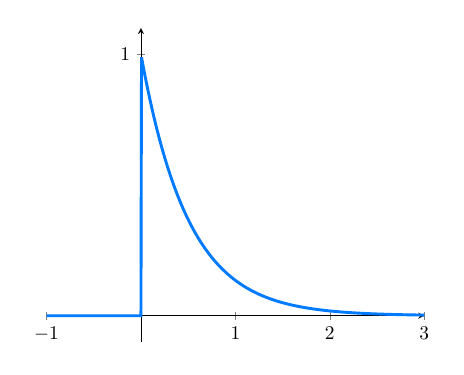
\begin{tikzpicture}[scale=0.7]
          \begin{axis}[
            xmin= -1, xmax= 3,
            ymin= -0.1, ymax = 1.1,
            axis lines = middle,
            ytick={1}, xtick={}
          ]
            \addplot[domain=-2:4, samples=1000, lightblue, line width=1.5]{x<0 ? 0: exp(-2*x)};
          \end{axis}
        \end{tikzpicture}
        \end{minipage} $\begin{array}{l}
          \begin{aligned}
            E_T&= \int_{-\infty}^{\infty} |x(t)|^2\dt=\int_{0}^{\infty} |e^{-2t} |^2\dt=\int_{0}^{\infty} e^{-4t}\dt\\
               &= \left[ -\dfrac{1}{4}e^{-4t}  \right] _0^{\infty}=-\dfrac{1}{4}\cdot [0-1]=\dfrac{1}{4}\mathrm{J} \\
          \end{aligned}\\
          P_m=\lim_{T \to \infty} \dfrac{1}{2T}=\int_{-T}^{T} |x(t)|^2\dt=\lim_{T \to \infty} \dfrac{E_T}{2T}=\dfrac{\frac{1}{4} }{+\infty}=0\mathrm{W} 
        \end{array}$
      \item \db{$x(t)=e^{j\left( 2t+\frac{\pi}{4}  \right) } $} 

        \begin{minipage}{0.3\textwidth}
          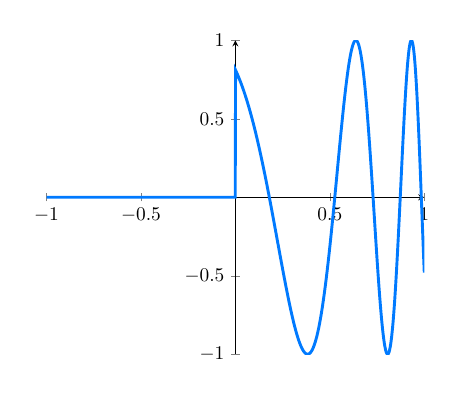
\begin{tikzpicture}[scale=0.7]
          \begin{axis}[
            xmin= -1, xmax= 1,
            ymin= -1, ymax = 1,
            axis lines = middle,
          ]
            \addplot[domain=-1:1, samples=1000, lightblue, line width=1.5]{x<0 ? 0 : sin(deg(exp(2*x+pi/4)))};
          \end{axis}
        \end{tikzpicture}
        \end{minipage}$\begin{aligned}
          E_T&= \int_{-\infty}^{\infty} |x(t)|^2\dt=\int_{-\infty}^{\infty} \left| e^{j\left(2t+\frac{\pi}{4} \right)}  \right|^2\dt    \\
             &= \int_{-\infty}^{\infty} 1^2\dt=[t] _{-\infty}^{\infty}=\infty-(-\infty)=\infty \\
             P_m&= \dfrac{1}{T}\int_{-\frac{T}{2} }^{\frac{T}{2} } \left| e^{j\left( 2t+\frac{\pi}{4}  \right) }  \right| ^2\dt=\dfrac{1}{T}\int_{-\frac{T}{2} }^{\frac{T}{2} } 1\dt   \\
                &= \dfrac{1}{T}\cdot [t]_{-\frac{T}{2} }^{\frac{T}{2} }=\dfrac{1}{T}\cdot \left( \dfrac{T}{2}-\left( -\dfrac{T}{2} \right)  \right) =\dfrac{1}{T}\cdot T=1 \\
        \end{aligned}$
      \item \db{$x(t)=\cos(t)$} 

        \begin{minipage}{0.3\textwidth}
          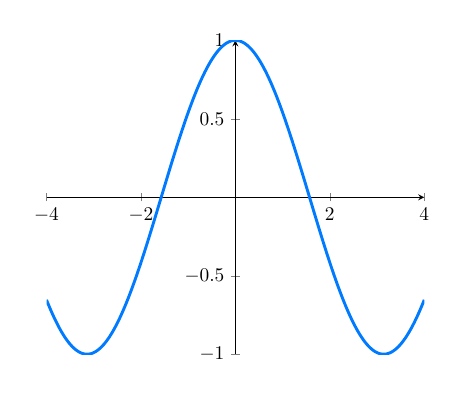
\begin{tikzpicture}[scale=0.7]
          \begin{axis}[
            xmin= -4, xmax= 4,
            ymin= -1, ymax = 1,
            axis lines = middle,
          ]
            \addplot[domain=-4:4, samples=1000, lightblue, line width=1.5]{cos(deg(x))};
          \end{axis}
        \end{tikzpicture}
        \end{minipage}$\begin{aligned}
          E_T&= \int_{-\infty}^{\infty} |x(t)|^2\dt=\int_{-\infty}^{\infty} |\cos(t)|^2\dt=\int_{-\infty}^{\infty} \cos^2(t)\dt    \\
          &= \dfrac{1}{2}\int_{-\infty}^{\infty} 1+\cos(2t)\dt=\dfrac{1}{2}\cdot \left[ t+\dfrac{1}{2}\sin(2t) \right]_{-\infty}^{\infty}   \\
          &=  \\
          P_m&= \dfrac{1}{T}\int_{-\frac{T}{2} }^{\frac{T}{2} } \cos^2(t)\dt=\dfrac{1}{2T}\left[ t+\dfrac{\sin(2t)}{2} \right] _{-\frac{T}{2} }^{\frac{T}{2} }  \\
          &= \dfrac{1}{2T}\left( \dfrac{T}{2}+\dfrac{t}{2}+\dfrac{\sin(T)-\sin(-T)}{2} \right) =\dfrac{1}{2T}\left( T+\tozero{\sin(T)}\:  \right)=\dfrac{1}{2}\mathrm{W}  \\
        \end{aligned}$
      \item \db{$x[n]=\left( \dfrac{1}{2} \right) ^nu[n]$} 

        \begin{minipage}{0.3\textwidth}
          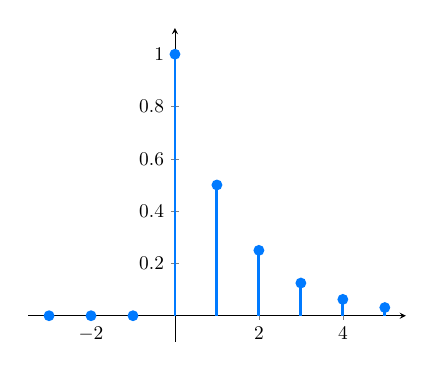
\begin{tikzpicture}[scale=0.7]
          \begin{axis}[
            xmin= -3.5, xmax= 5.5,
            ymin= -0.1, ymax = 1.1,
            axis lines = middle,
          ]
          \addplot[line width=1.5, lightblue, ycomb, mark=*] coordinates {
              (-3,0) (-2,0) (-1,0) (0, 1) (1, 0.5) (2,0.25) (3,0.125) (4, 0.0625) (5, 0.03125)
            };
          \end{axis}
        \end{tikzpicture}
        \end{minipage}$\begin{aligned}
        E_T&= \sum_{n=-\infty}^{\infty} |x[n]|^2=\sum_{n=0}^{\infty} \left| \left( \dfrac{1}{2} \right) ^n \right| ^2=\sum_{n=0}^{\infty} \left( \dfrac{1}{2} \right) ^{2n} \\
        &= \sum_{n=0}^{\infty} \left( \dfrac{1}{4} \right) ^n=\dfrac{1-0\cdot \frac{1}{4} }{1-\frac{1}{4} }=\dfrac{4}{3}\mathrm{J} \\
        P_m&= \lim_{N \to \infty} \dfrac{E_T}{2N+1}=\dfrac{\frac{4}{3} }{+\infty}=0\mathrm{W} \\
        \end{aligned}$
      \item \db{$x[n]=e^{j\left( \frac{\pi}{2} n+\frac{\pi}{8}  \right) } $} 

        \begin{minipage}{0.45\textwidth}
          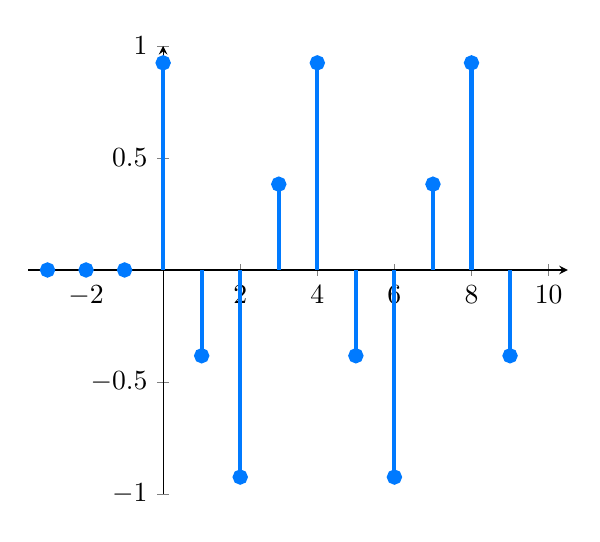
\begin{tikzpicture}
          \begin{axis}[
            xmin= -3.5, xmax= 10.5,
            ymin= -1, ymax = 1,
            axis lines = middle,
          ]
          \addplot[lightblue, line width=1.5, ycomb, mark=*] coordinates {
              (-3, -0.0)
              (-2, -0.0)
              (-1, 0.0)
              (0, 0.9238795325112867)
              (1, -0.3826834323650897)
              (2, -0.9238795325112868)
              (3, 0.38268343236509)
              (4, 0.9238795325112867)
              (5, -0.3826834323650899)
              (6, -0.9238795325112867)
              (7, 0.3826834323650898)
              (8, 0.9238795325112867)
              (9, -0.38268343236508967)
            };
          \end{axis}
        \end{tikzpicture}
        \end{minipage}$\begin{aligned}
        E_T&= \sum_{n=-\infty}^{\infty} |x[n]|^2=\sum_{n=0}^{\infty} \left| e^{j\left( \frac{\pi}{2} n+\frac{\pi}{8}  \right) }  \right| ^2=\sum_{n=0}^{\infty} 1^2=\infty \\
        P_m&= \dfrac{1}{N}\sum_{n=0}^{N-1} |x[n]|^2=\left\{ \omega_0=\dfrac{\pi}{2}\to N=\dfrac{2\pi}{\frac{\pi}{2} }k=4k\underset{k=1}{=} 4\right\}  \\
        &= \dfrac{1}{4}\sum_{n=0}^{3} 1^2=\dfrac{4}{4}=1\mathrm{W} \\
        \end{aligned}$
      \item \db{$x[n]=\cos\left( \dfrac{\pi}{4}n \right)u[n] $} 

        \begin{minipage}{0.45\textwidth}
        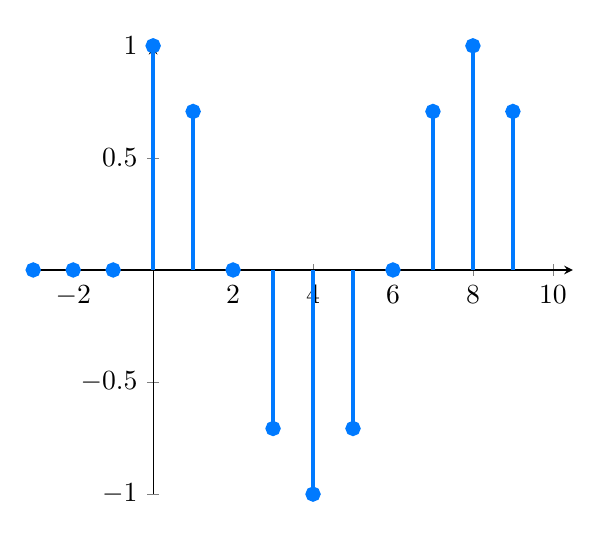
\begin{tikzpicture}
          \begin{axis}[
            xmin= -3, xmax= 10.5,
            ymin= -1, ymax = 1,
            axis lines = middle,
          ]
          \addplot[lightblue, line width=1.5, ycomb, mark=*] coordinates {
              (-3, -0.0)
              (-2, 0.0)
              (-1, 0.0)
              (0, 1.0)
              (1, 0.7071067811865476)
              (2, 6.123233995736766e-17)
              (3, -0.7071067811865475)
              (4, -1.0)
              (5, -0.7071067811865477)
              (6, -1.8369701987210297e-16)
              (7, 0.7071067811865474)
              (8, 1.0)
              (9, 0.7071067811865477)
            };
          \end{axis}
        \end{tikzpicture}
        \end{minipage}$\begin{aligned}
        E_T&= \sum_{n=-\infty}^{\infty} |x[n]|^2=\sum_{n=0}^{\infty} \left| \cos\left( \dfrac{\pi}{4}n \right)  \right| ^2=\infty \\
        P_m&= \dfrac{1}{N}\sum_{n=0}^{N-1}|x[n]|^2=\left\{ \omega_0=\dfrac{\pi}{4}\to N=\dfrac{2\pi}{\frac{\pi}{4} }k=8k\underset{k=1}{=}8 \right\}   \\
        &= \dfrac{1}{8}\sum_{n=0}^{7} \dfrac{1}{2}\left[ 1+\tozero{\cos(2n)} \: \right] =\dfrac{8}{16}+0=\dfrac{1}{2}\mathrm{W} \\
        \end{aligned}$
\end{enumerate}
  \item \lb{Considere una señal $x[n]$ en la que  $x[n]=0$ para  $n<-2$ y  $n>4$. Para cada una de las señales siguientes determine los valores de  $n$ en los que se garantiza que la señal es cero.}
    \begin{center}
      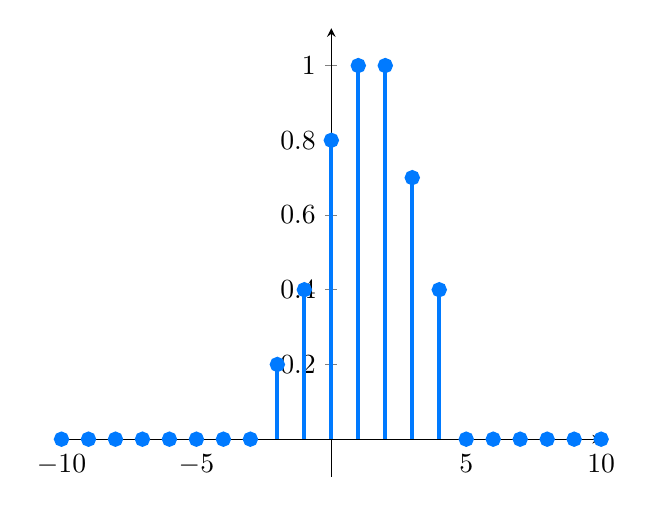
\begin{tikzpicture}
        \begin{axis}[
          xmin= -10, xmax= 10,
          ymin= -0.1, ymax = 1.1,
          axis lines = middle
        ]
        \addplot[lightblue, line width=1.5, ycomb, mark=*] coordinates {
 (-10, 0.0)
(-9, 0.0)
(-8, 0.0)
(-7, 0.0)
(-6, 0.0)
(-5, 0.0)
(-4, 0.0)
(-3, 0.0)
(-2, 0.2)
(-1, 0.4)
(0, 0.8)
(1, 1.0)
(2, 1.0)
(3, 0.7)
(4, 0.4)
(5, 0.0)
(6, 0.0)
(7, 0.0)
(8, 0.0)
(9, 0.0)
(10, 0.0)       

          };
        \end{axis}
      \end{tikzpicture}
    \end{center}
    \begin{enumerate}[label=\color{red}\textbf{\alph*)}]
      \item  \db{$x[n-3]$} 
      
        \begin{minipage}{0.45\textwidth}
       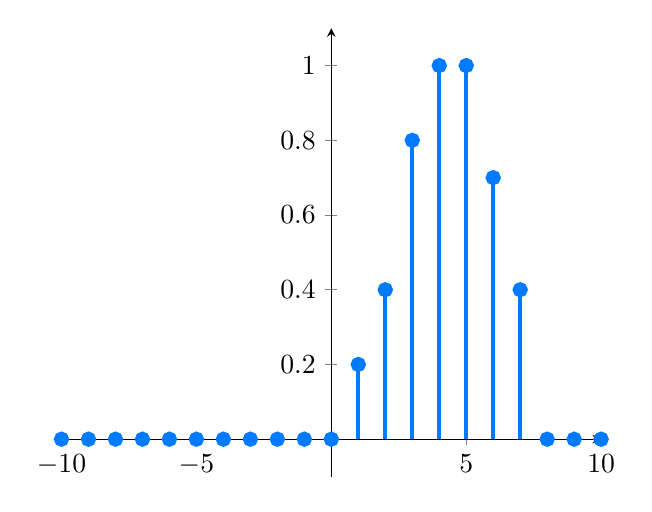
\begin{tikzpicture}
        \begin{axis}[
          xmin= -10, xmax= 10,
          ymin= -0.1, ymax = 1.1,
          axis lines = middle,
        ]
        \addplot[lightblue, line width=1.5, ycomb, mark=*] coordinates {
(-10, 0.0)
(-9, 0.0)
(-8, 0.0)
(-7, 0.0)
(-6, 0.0)
(-5, 0.0)
(-4, 0.0)
(-3, 0.0)
(-2, 0.0)
(-1, 0.0)
(0, 0.0)
(1, 0.2)
(2, 0.4)
(3, 0.8)
(4, 1.0)
(5, 1.0)
(6, 0.7)
(7, 0.4)
(8, 0.0)
(9, 0.0)
(10, 0.0)
          };
        \end{axis}
      \end{tikzpicture}
 
        \end{minipage}\qquad \begin{minipage}{0.45\textwidth}
        Vemos que esta señal se corresponde con un desplazamiento de 3 unidades a la derecha. Por tanto, $x[n-3]=0$ para  $n<1$ y  $n>7$.
        \end{minipage}
      \item \db{$x[n+4]$}
      
 \begin{minipage}{0.45\textwidth}
       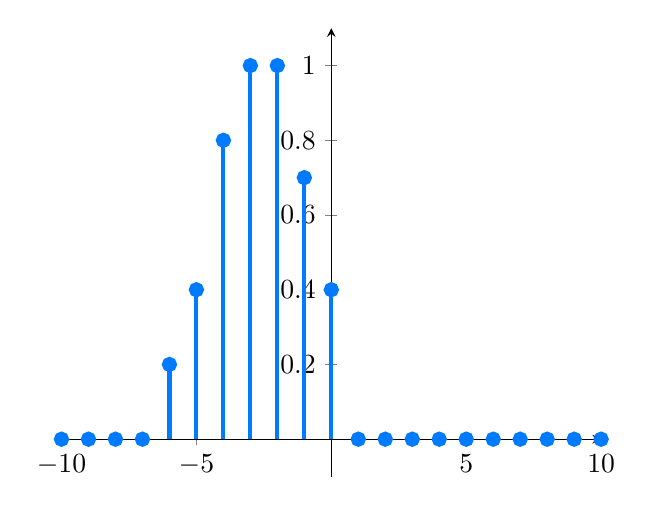
\begin{tikzpicture}
        \begin{axis}[
          xmin= -10, xmax= 10,
          ymin= -0.1, ymax = 1.1,
          axis lines = middle
        ]
        \addplot[lightblue, line width=1.5, ycomb, mark=*] coordinates {
(-10, 0.0)
(-9, 0.0)
(-8, 0.0)
(-7, 0.0)
(-6, 0.2)
(-5, 0.4)
(-4, 0.8)
(-3, 1.0)
(-2, 1.0)
(-1, 0.7)
(0, 0.4)
(1, 0.0)
(2, 0.0)
(3, 0.0)
(4, 0.0)
(5, 0.0)
(6, 0.0)
(7, 0.0)
(8, 0.0)
(9, 0.0)
(10, 0.0)
          };
        \end{axis}
      \end{tikzpicture}
 
        \end{minipage}\qquad \begin{minipage}{0.45\textwidth}
        Vemos que la señal se corresponde con un desplazamineto de 4 unidades a la izquierda. Por tanto $x[n+4]=0$ para  $n<-6$ y  $n>0$.
        \end{minipage}

      \item \db{$x[-n]$} 
      
 \begin{minipage}{0.45\textwidth}
       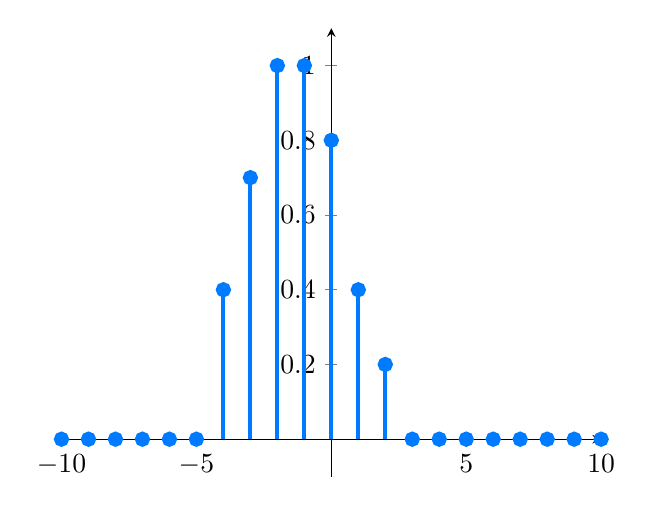
\begin{tikzpicture}
        \begin{axis}[
          xmin= -10, xmax= 10,
          ymin= -0.1, ymax = 1.1,
          axis lines = middle
        ]
        \addplot[lightblue, line width=1.5, ycomb, mark=*] coordinates {
(-10, 0.0)
(-9, 0.0)
(-8, 0.0)
(-7, 0.0)
(-6, 0.0)
(-5, 0.0)
(-4, 0.4)
(-3, 0.7)
(-2, 1.0)
(-1, 1.0)
(0, 0.8)
(1, 0.4)
(2, 0.2)
(3, 0.0)
(4, 0.0)
(5, 0.0)
(6, 0.0)
(7, 0.0)
(8, 0.0)
(9, 0.0)
(10, 0.0)
          };
        \end{axis}
      \end{tikzpicture}
 
        \end{minipage}\qquad \begin{minipage}{0.45\textwidth}
        Vemos que est señal se corresponde con una reflexión o simetría de la señal con respecto al eje central. Por tanto, $x[-n]=0$ para  $n<-4$ y  $n>2$.
        \end{minipage}

      \item \db{$x[-n+2]$} 

 \begin{minipage}{0.45\textwidth}
       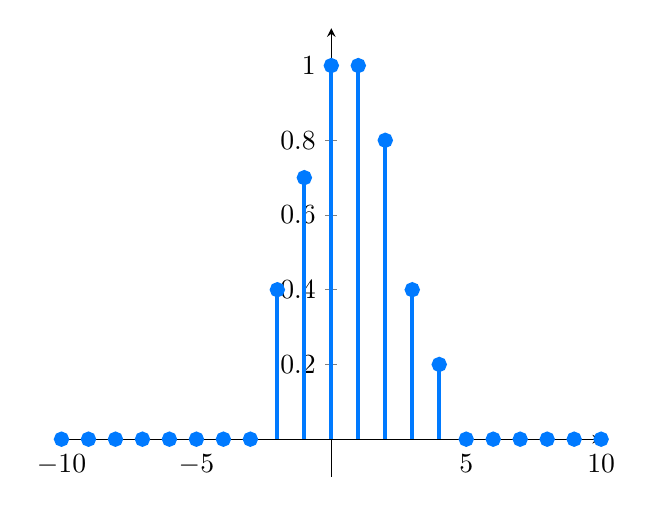
\begin{tikzpicture}
        \begin{axis}[
          xmin= -10, xmax= 10,
          ymin= -0.1, ymax = 1.1,
          axis lines = middle  
        ]
        \addplot[lightblue, line width=1.5, ycomb, mark=*] coordinates {
(-10, 0.0)
(-9, 0.0)
(-8, 0.0)
(-7, 0.0)
(-6, 0.0)
(-5, 0.0)
(-4, 0.0)
(-3, 0.0)
(-2, 0.4)
(-1, 0.7)
(0, 1.0)
(1, 1.0)
(2, 0.8)
(3, 0.4)
(4, 0.2)
(5, 0.0)
(6, 0.0)
(7, 0.0)
(8, 0.0)
(9, 0.0)
(10, 0.0)
          };
        \end{axis}
      \end{tikzpicture}
 
        \end{minipage} \begin{minipage}{0.45\textwidth}
        Vemos que esta señal se corresponde con una reflexión o simetría de la señal con respecto al eje central y un desplazamiento a la derecha de 2 unidades. Por tanto, $x[-n+2]=0$, para  $n<-2$ y  $n>4$
        \end{minipage}

      \item \db{$x[-n-2]$} 

 \begin{minipage}{0.45\textwidth}
       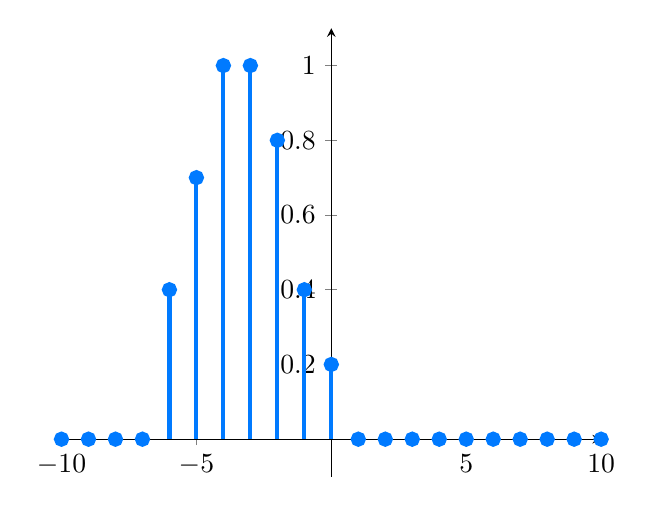
\begin{tikzpicture}
        \begin{axis}[
          xmin= -10, xmax= 10,
          ymin= -0.1, ymax = 1.1,
          axis lines = middle,     
        ]
        \addplot[lightblue, line width=1.5, ycomb, mark=*] coordinates {
(-10, 0.0)
(-9, 0.0)
(-8, 0.0)
(-7, 0.0)
(-6, 0.4)
(-5, 0.7)
(-4, 1.0)
(-3, 1.0)
(-2, 0.8)
(-1, 0.4)
(0, 0.2)
(1, 0.0)
(2, 0.0)
(3, 0.0)
(4, 0.0)
(5, 0.0)
(6, 0.0)
(7, 0.0)
(8, 0.0)
(9, 0.0)
(10, 0.0)
          };
        \end{axis}
      \end{tikzpicture}
 
        \end{minipage} \begin{minipage}{0.45\textwidth}
        Vemos que esta señal se corresponde con una reflexión o simetría de la señal con respecto al eje central y un desplazamiento a la izquierda de 2 unidades. Por tanto, $x[-n-2]=0$, para  $n<-6$ y  $n>0$.
        \end{minipage}

    \end{enumerate}
  \item \lb{Considere una señal $x(t)$ en la que  $x(t)=0$ para  $t<3$. Para cada una de las señales siguientes deteremine los valores de $t$ en los que se garantiza que la señal es cero.}
\begin{center}
\includegraphics[width=0.7\linewidth]{"Ejercicio 5/Figure 1"}
\end{center}
    \begin{enumerate}[label=\color{red}\textbf{\alph*)}]
      \item \db{$x(1-t)$} 

\begin{minipage}{0.45\textwidth}
\includegraphics[width=\linewidth]{"Ejercicio 5/Figure 2"}
\end{minipage} \begin{minipage}{0.45\textwidth}
Podemos expresar dicha señal de la forma $x(-t+1)$, donde vemos rápidamente que se trata de una inversión y de un desplazamiento de un segundo hacia la derecha. Por lo tanto, como se muestra en la figura, la señal  $x(1-t)$ será cero para  $t\ge -2$.
\end{minipage}

      \item \db{$x(1-t)+x(2-t)$} 

\begin{minipage}{0.45\textwidth}
\includegraphics[width=\linewidth]{"Ejercicio 5/Figure 3"} 
\end{minipage}\begin{minipage}{0.45\textwidth}
Si la señal $x(1-t)$ es cero para  $t\ge -2$, vemos fácilmente que $x(2-t)$ es cero para  $t\ge -1$. Por lo tanto, al sumarlas, seguirá siendo cero para $t\ge -1$.
\end{minipage}

      \item \db{$x(1-t)x(2-t)$} 
      
      \begin{minipage}{0.45\textwidth}
      \includegraphics[width=\linewidth]{"Ejercicio 5/Figure 4"}
      \end{minipage} \begin{minipage}{0.45\textwidth}
      Si la señal $x(1-t)$ es cero para  $t\ge -2$, vemos fácilmente que $x(2-t)$ es cero para  $t\ge -1$. Por lo tanto, al multiplicarlas, seguirá ´siendo cero para $t\ge -2$.
      \end{minipage}

      \item \db{$x(3t)$} 
      
      \begin{minipage}{0.45\textwidth}
      \includegraphics[width=\linewidth]{"Ejercicio 5/Figure 5"}
      \end{minipage} \begin{minipage}{0.45\textwidth}
      Si la señal $x(t)$ es cero para  $t<3$, al aplicar la compresión por el factor  $a=3$, la señal  $x(3t)$ será cero para  $t>1$.
      \end{minipage}

      \item \db{$x\left( \dfrac{t}{3} \right) $} 

\begin{minipage}{0.45\textwidth}
\includegraphics[width=\linewidth]{"Ejercicio 5/Figure 6"}
\end{minipage} \begin{minipage}{0.45\textwidth}
Si la señal $x(t)$ es cero para  $t<3$, al aplicar la expansión por el factor  $a=\dfrac{1}{3}$, la señal $x\left( \dfrac{t}{3} \right) $ será cero para $t>9$.
\end{minipage}
    \end{enumerate}
  \item \lb{Determine si cada de las siguientes señales es periódica:}
    \begin{enumerate}[label=\color{red}\textbf{\alph*)}]
      \item \db{$x(t)=2e^{j\left( t+\frac{\pi}{4}  \right)u(t) } $} 

        \begin{itemize}[label=\textbullet]
          \item La parte exponencial $\left( e^{j\left( t+\frac{\pi}{4}  \right) }  \right) $ es un señal compleja con una frecuencia $\omega_0=1$, lo cual sugiere periodicidad.
          \item Sin embargo, la función escalón $u(t)$ hace que la señal solo existe para  $t\ge 0$. Esto significa que la señal no se repite en todo el dominio de $t$, por lo tanto, no es periódica.
        \end{itemize}
      \item \db{$x(t)=x[n]=e[n]+u[-n]$} 
        \begin{itemize}[label=\textbullet]
          \item $u[n]$ es la función escalón, que es 1 para  $n\ge 0$ y $0$ para  $n<0$.
          \item  $u[-n]$ es la función escalón reflejada, que es 1 para $n\le 0$ y 0 para $n>0$.
          \item Sumando ambas funciones: la señal es 1 para todo  $n$, es decir,  $x[n]=1$ para todo  $n$, esto hace que la señal sea constante, por lo tanto, es periódica para cualquier período  $N$.
        \end{itemize}
      \item \db{$x[n]=\sum_{k=-\infty}^{\infty} (\delta[n-4k]-\delta[n-1-4k])$}  
        \begin{itemize}[label=\textbullet]
          \item La señal está compuesta por dos deltas desplazadas en el tiempo.
          \item la forma general es de dos impulsos cada intervalo de 4 muestras.
          \item Por lo tanto, la señal es periódica con período $N=4$.
        \end{itemize}
    \end{enumerate}
  \item \lb{Para cada una de las señales siguientes determine los valores de la variable independiente en los que se garantice que la parte par de la señal es cero.}
    \begin{enumerate}[label=\color{red}\textbf{\alph*)}]
      \item \db{$x[n]=u[n]-u[n-4]$} 

        Esta señal es un tren de impulsos rectangular con valores de 1, en $0\le n\le 3$ y 0 en otros lugares.
        \begin{itemize}[label=\textbullet]
          \item Antisimetría respecto a $n=\dfrac{3}{2}$, por lo que su parte par será cero en los puntos donde $x[n]=-x[-n]$.
          \item Para $n=0,1,2,3$ tenemos valores de 1.
          \item Para  $n=-1,-2,-3$, la función es 0.
          \item La parte par será cero en los valores fuera del intervalo  $[-3,3]$.
        \end{itemize}
      \item $\db{x(t)=\sin\left( \dfrac{t}{2} \right) } $ 

        La función seno es impar, es decir: \[
        \sin\left( \dfrac{t}{2} \right) +\sin\left( \dfrac{t}{2} \right) =0
        \] 
        Por definición, su parte par es cero para todo $t$.
      \item \db{$x[n]=\left( \dfrac{1}{2} \right) ^nu[n-3]$}

        Esta señal es una secuencia geométrica desplazada a partir de $n=3$, es decir:  \[
          x[n]=\begin{cases}
            \left( \dfrac{1}{2} \right) ^{n} & \text{si }n\ge 3\\
            0 & \text{en otro caso}
          \end{cases}
        \] 
        Para que su parte par sea cero, debe cumplirse $x[n]=-x[-n]$, pero como la función es unilateral, su parte par será cero donde  $x[n]=0$, es decir, donde  $n<3$.
      \item \db{$x(t)=e^{-5t}u(t+2) $} 

        Esta señal es una exponencial decreciente activada en $t\ge -2$.
        \begin{itemize}[label=\textbullet]
          \item Es unilateral y no tiene valores negativos simétricos, por lo que su parte par será cero antes de la activación, es decir, cuando $t\le -2$.
        \end{itemize}
    \end{enumerate}
  \item \lb{Exprese la parte real de cada una de las siguientes señales de la forma $Ae^{-at}\cos(\omega t+\varphi) $, donde $A,a,\omega$ y $\varphi$ son números reales con $A\ge 0$ y $-\pi\le \varphi\le \pi$.} 
    \begin{enumerate}[label=\color{red}\textbf{\alph*)}]
      \item \db{$x(t)=-2$} 
        \[
        x(t)=2e^{-0t}\cos(0t+\pi), 
        \] donde: \[
        \begin{array}{ll}
          \bullet\, A=2 & \bullet\, \omega=0\\
          \bullet\, a=0 & \bullet\, \varphi=\pi
        \end{array}
        \] 
      \item \db{$x(t)=\sqrt{2} e^{j\frac{\pi}{4} } \cos(3t+2\pi)$} 

        $x(t)=\sqrt{2} e^{j\frac{\pi}{4} } \cos(\lbb{3t+2\pi}{\theta+2\pi=\theta})=\sqrt{2}\left( \cos\left( \dfrac{\pi}{4} \right) +j\cdot \sin\left( \dfrac{\pi}{4} \right)  \right) \cos(3t)=(1+j)\cos(3t)$

        Solo tomamos la parte real, por lo que: \[
        x(t)=\cos\left( 3t+\dfrac{\pi}{4} \right) ,
        \] donde: \[
        \begin{array}{ll}
          \bullet\, A=1 & \bullet\, \omega=3\\
          \bullet\, a=0 & \bullet\,\varphi=\dfrac{\pi}{4}
        \end{array}
        \] 
      \item \db{$x(t)=e^{-t}\sin(3t+\pi) $} 

        Usaremos la identidad: \[
        \sin(\theta)=\cos\left( \theta-\dfrac{\pi}{2} \right) ,
        \] por lo que: \[
        x(t)=e^{-t}\cos\left( 3t+\pi-\dfrac{\pi}{2} \right) =e^{-t}\cos\left( 3t+\dfrac{\pi}{2} \right)   ,
        \] donde: \[
        \begin{array}{ll}
          \bullet\, A=1 & \bullet\,\omega=3\\
          \bullet\, a=1 & \bullet\, \varphi=\dfrac{\pi}{2}
        \end{array}
        \] 
      \item \db{$x(t)=je^{(-2+j 100)t} $} 
    \end{enumerate}
  \item \lb{Determine si cada una de las siguientes señales es periódica. En caso afirmativo especifique su periodo fundamental.}
    \begin{enumerate}[label=\color{red}\textbf{\alph*)}]
      \item \db{$x(t)=-2$} 

        La señal tiene la forma $x(t)=e^{j\omega t} $, que es periódica si la frecuencia angular $\omega$ es un múltiplo racional de $2\pi$: \[
        \omega=10.
        \] 
        El periodo fundamental es: \[
        T=\dfrac{2\pi}{\omega}=\dfrac{2\pi}{10}=\dfrac{\pi}{5}.
        \] 
        La señal es periódica con periodo fundamental $T=\dfrac{\pi}{5}$.
      \item \db{$x(t)=e^{(-1+j)t} $} 

        Esta señal tiene un término $e^{-t} $, que representa un decrecimiento exponencial. Si hay un término exponencial con un exponente real negativo, la señal nunca se repite exactamente, ya que disminuye continuamente, por lo tanto, no es periódica.
      \item \db{$x[n]=e^{j 7\pi n} $} 

        $\omega=7\pi\longrightarrow N=\dfrac{2\pi}{\omega}\cdot m=\dfrac{2\pi}{7\pi}\cdot m=\dfrac{2}{7}\cdot m\longrightarrow N=2\:(m=7)$

        La señal es periódica, con periodo fundamental $N=2$.
      \item \db{$x[n]=3e^{j3\pi\frac{n+\frac{1}{2} }{5} } $} 

        $\omega=\dfrac{2\pi}{5}\longrightarrow N=\dfrac{2\pi}{\omega}\cdot m=\dfrac{2\pi}{\frac{3\pi}{5} }\cdot m=\dfrac{10}{3}\cdot m\longrightarrow N=10\:(m=3)$
      \item \db{$x[n]=3e^{j\frac{3}{5} \left( n+\frac{1}{2}  \right) } $} 

        $\omega=\dfrac{3}{5}\longrightarrow N=\dfrac{2\pi}{\omega}\cdot m=\dfrac{2\pi}{\frac{3}{5} }\cdot m=\dfrac{10\pi}{3}\cdot m\longrightarrow $ No se puede.

        La señal no es periódica.
    \end{enumerate}
  \item \lb{Determine el periodo fundamental de la señal $x(t)=2\cos(10t+1)-\sin(4t-1)$.} 

        Para determinar el \textbf{periodo fundamental} de la señal $x(t)=2\cos(10t+1)-\sin(4t-1)$, debemos analizar los periodos de las componentes individuales de la señal y encontrar el \textbf{mínimo común múltiplo} de estos periodos.
        \begin{enumerate}[label=Paso \arabic*:]
            \item Identificar las frecuencias angulares

                La señal está compuesta por dos términos:
                \begin{itemize}[label=\textbullet]
                    \item $2\cos(10t+1)$: Su frecuencia angular es $\omega_1=10$.
                    \item $-\sin(4t-1)$: Su frecuencia angular es $\omega_2=4$.
                \end{itemize}
                El periodo de una señal está relacionado con su frecuencia angular mediante la fórmula: \[
                T=\dfrac{2\pi}{\omega}.
                \] 
            \item Calcular los periodos de las componentes
                \begin{itemize}[label=\textbullet]
                    \item Para $\omega_1=10$, el periodo es: \[
                    R=\dfrac{2\pi}{10}=\dfrac{\pi}{5}.
                    \] 
                \item Para $\omega_2=4$, el periodo es: \[
                T_2=\dfrac{2\pi}{4}=\dfrac{\pi}{2}.
                \] 
                \end{itemize}
            \item Encontrar el periodo fundamental

                El periodo fundamental de la señal compuesta es el \textbf{mínimo común múltiplo} de los periodos $T_1$ y $T_2$. Para encontrarlo, debemos expresar ambos periodos como fracciones con el mismo denominador: \[
                T_1=\dfrac{\pi}{5},\quad T_2=\dfrac{\pi}{2}\longrightarrow T_1=\dfrac{2\pi}{10},\quad T_2=\dfrac{5\pi}{10}.
                \]  
                El \textbf{mcm} de $\dfrac{2\pi}{10}$ y $\dfrac{5\pi}{10}$ es $\dfrac{10\pi}{10}=\pi$.
        \end{enumerate}
        El periodo fundamental de la señal $x(t)$ es:  \[
        T=\pi.
        \] 
  \item \lb{Determine el periodo fundamental de la señal $x[n]=1+e^{j\frac{4\pi n}{7}}-e^{j\frac{2\pi n}{5} }$.}

      Para determinar el periodo fundamental de la señal \[x[n]=1+e^{j\frac{4\pi n}{7}}-e^{j\frac{2\pi n}{5} },\] debemos analizar la periodicidad de cada término.
       \begin{itemize}[label=\textbullet]
          \item El término constante 1 es periódico con cualquier periodo.
          \item En el término $e^{j\frac{4\pi n}{4} } $, buscamos $N$ tal que \[
          e^{j\frac{4\pi(n+N)}{7} } =e^{j\frac{4\pi n}{7} } ,
          \] lo que implica \[
          e^{j\frac{4\pi N}{7} } =1.
          \] 
          Esto es cierto cuando \[
          \dfrac{4\pi N}{7}=2\pi k,\quad k\in \Z.
          \] 
          De aquí se obtiene \[
          N=\dfrac{7k}{2}.
          \] 
          Se requiere que $N$ sea entero, por lo que el menor $k$ que cumple esto es $k=2$, dando $N=7$.
      \item Para el término  $-e^{j\frac{2\pi n}{5} } $, se sigue un razonamiento similar. Se busca $N$ tal que \[
      e^{j\frac{2\pi(n+N)}{5} } =e^{j\frac{2\pi n}{5} } ,
      \] lo que requiere \[
      e^{j\frac{2\pi N}{5} } =1.
      \] 
      Esto se cumple si \[
      \dfrac{2\pi N}{5}=2\pi m,\quad m\in \Z,
      \] y de donde se obtiene \[
      N=5m.
      \] El mínimo $m=1$ nos da  $N=5$.
      \end{itemize}
      La señal completa $x[n]$ es la suma de componentes periódicas con periodos 7 y 5. El periodo fundamental de  $x[n]$ será el mínimo común múltiplo entre 7 y 5, que es  \[
      N=\mathrm{lcm}(7,5)=35.
      \] 
      Por lo tanto, el periodo fundamental de la señal es \textbf{35}. 
  \item \lb{Considere la señal en tiempo discreto $x[n]=1-\sum_{k=3}^{\infty} \delta[n-1-k]$. Determine los valores de los números enteros $M$ y  $n_0$ que permiten que $x[n]$ pueda expresarse como  $x[n]=u[Mn+n_0]$} 

      \begin{enumerate}[label=Paso \arabic*:]
          \item Analicemos la señal

              El término 1 indica que $x[n]$ comienza con un valor inicial de 1. El segundo término, $-\sum_{k=3}^{\infty} \delta[n-1-k]$, representa una suma de deltas desplazadas, que restan 1 en ciertos valores de $n$. Específicamente, el índice de cada delta es: \[
              n=1+k,\quad k\ge 3.
              \] 
              Sustituyendo $k=3,4,5,\dots$, obtenemos los valores de $n$ donde las deltas están activas: \[
              n=4,5,6,\dots
              \] 
              Por lo tanto, la señal $x[n]$ se puede describir como:  \[
                  x[n]=\begin{cases}
                      1, & n<4\\
                      0, & n\ge 4
                  \end{cases}
              \] 
              Esto significa que $x[n]$ es una señal que vale 1 para  $n<4$ y 0 para  $n\ge 4$.
          \item Relación con $u[Mn+n_0]$

              La función escalón unitario $u[n]$ está definida como:  \[
                  u[n]=\begin{cases}
                      1, & n\ge 0\\
                      0, & n<0
                  \end{cases}
              \] 
              Queremos expresar $x[n]$ en la forma  $x[n]=u[Mn+n_0]$. Esto implica que debemos encontrar valores de $M$ y $n_0$ tales que: \[
                  u[Mn+n_0]=\begin{cases}
                      1, & n<4\\
                      0, & n\ge 4
                  \end{cases}
              \] 
              Para que esto sea cierto, el argumento el escalón unitario debe cambiar de signo en $n=4$. Específicamente:
               \begin{itemize}[label=\textbullet]
                   \item Para $n<4$, queremos que  $Mn+n_0<0$, lo que asegura que $u[Mn+n_0]=1$.
                   \item Para $n\ge 4$, queremos que $Mn+n_0\ge 0$, lo que asegura que $u[Mn+n_0]=0$.
              \end{itemize}
          \item Determinación de $M$ y  $n_0$

              El cambio ocurre en $n=4$, por lo que imponemos la condición de igualdad en el argumento del escalón:  \[
              M(4)+n_0=0\longrightarrow n_0=-4M.
              \] 
              Para que $u[Mn+n_0]$ sea válido, $M$ debe ser negativo (ya que queremos que el escalón sea 1 para $n<4$ y 0 para  $n\ge 4$). Tomemos $M=-1$. Sustituyendo en la ecuación anterior:  \[
              n_0=-4(-1)=4.
              \] 
              Por lo tanto, los valores son: \[
              M=-1,\quad n_0=4.
              \] 
          \item Verificación

              Sustituimos $M=-1$ y  $n_0=4$ en $u[Mn+n_0]$: \[
                  u[Mn+n_0]=u[-n+4].
              \] 
              \begin{itemize}[label=\textbullet]
                  \item Para $n<4,-n+4>0$, por lo que  $u[-n+4]=1$.
                  \item Para  $n\ge 4,-n+4\le 0$, por lo que $u[-n-4]=0$.
              \end{itemize}
              Esto coincide exactamente con $x[n]$. Por lo tanto, la señal puede expresarse como:  \[
                  x[n]=u[-n+4].
              \] 
              Los valores son: \[
              M=-1,\quad n_0=4.
              \] 
      \end{enumerate}
  \item \lb{Considere la señal en tiempo continuo $x(t)=\delta(t+2)-\delta(t+2)$. Calcule la energía de la señal  $y(t)=\int_{-\infty}^{t} x(\tau)\mathrm{d}\tau $.}

      Dada la señal en tiempo continuo: \[
      x(t)=\delta(t+2)-\delta(t+2),
      \] es evidente que $x(t)=0$, ya que los términos se cancelan entre sí.

      Ahora, se nos pide calcular la energía de la señal $y(t)$, donde: \[
      y(t)=\int_{-\infty}^{t} x(\tau)\mathrm{d}\tau. 
      \] 
      \begin{enumerate}[label=Paso \arabic*:]
          \item Calcular $y(t)$

              Dado que  $x(t)=0$, la integral de  $x(\tau)$ también será cero para cualquier  $t$. Por lo tanto:  \[
              y(t)=\int_{-\infty}^{t} 0\mathrm{d}+\tau=0 .
              \] 
          \item Energía de la señal $y(t)$

              La energía de un señal  $y(t)$ se define como: \[
              E_y=\int_{-\infty}^{\infty} |y(t)|^2\dt=\int_{-\infty}^{\infty} |0|^2\dt=\int_{-\infty}^{\infty} 0\dt=0  . 
              \] 
      \end{enumerate}
  \item \lb{La figura 1 muestra la señal continua $x(t)$. Represente cada una de las siguientes señales.}
    \begin{center}
      \begin{tikzpicture}[scale=1.5]
        \draw (-2.5,0) -- (2.5,0) node[right] {$t$};
        \draw (0,-1.5) -- (0,2.5) node[above] {$x(t)$};
        \draw[lightblue, line width=1.5] (-2, 0) -- (-2,-1) -- (-1,0) -- (-1, 1) -- (0,1) -- (0,2) -- (1,2) -- (1,1) -- (2,0);
        \foreach \x in {-2,...,2} {\node[below] at (\x,0) {$\x$};}
        \foreach \y in {-1, 1} {\node[right] at (0,\y) {$\y$};}
        \node[left] at (0,2) {$2$};
      \end{tikzpicture}\\
      \lb{Figura 1} 
    \end{center}
    \begin{enumerate}[label=\color{red}\textbf{\alph*)}]
      \item \db{$x(t-1)$} 
\begin{center}
      \begin{tikzpicture}[scale=1.5]
        \draw (-2.5,0) -- (3.5,0) node[right] {$t$};
        \draw (0,-1.5) -- (0,2.5) node[above] {$x(t-1)$};
        \draw[lightblue, line width=1.5] (-1, 0) -- (-1,-1) -- (0,0) -- (0, 1) -- (1,1) -- (1,2) -- (2,2) -- (2,1) -- (3,0);
        \foreach \x in {-2,...,3} {\node[below] at (\x,0) {$\x$};}
        \foreach \y in {-1, 1} {\node[right] at (0,\y) {$\y$};}
        \node[left] at (0,2) {$2$};
      \end{tikzpicture}
    \end{center}
      \item \db{$x(2-t)$} 
\begin{center}
      \begin{tikzpicture}[scale=1.5]
        \draw (-2.5,0) -- (4.5,0) node[right] {$t$};
        \draw (0,-1.5) -- (0,2.5) node[above] {$x(2-t)$};
        \draw[lightblue, line width=1.5] (0,0) -- ( 1,1) -- (1,2) -- (2,2) -- (2,1) -- (3,1) -- (3,0) -- (4,-1) -- (4,0);
        \foreach \x in {-2,...,4} {\node[below] at (\x,0) {$\x$};}
        \foreach \y in {-1, 1} {\node[right] at (0,\y) {$\y$};}
        \node[left] at (0,2) {$2$};
      \end{tikzpicture}
    \end{center}
      \item \db{$x(2t+1)$} 
\begin{center}
      \begin{tikzpicture}[scale=1.5]
        \draw (-2.5,0) -- (2.5,0) node[right] {$t$};
        \draw (0,-1.5) -- (0,2.5) node[above] {$x(2t+1)$};
        \draw[lightblue, line width=1.5] (-1.5, 0) -- (-1.5,-1) -- (-1,0) -- (-1,1) -- (-0.5,1) -- (-0.5, 2) -- (0,2) -- (0,1) -- (0.5,0);
        \foreach \x in {-2,...,2} {\node[below] at (\x,0) {$\x$};}
        \foreach \y in {-1, 1, 2} {\node[left] at (0,\y) {$\y$};}
      \end{tikzpicture}
    \end{center}
      \item \db{$x\left( 4-\dfrac{t}{2} \right) $} 
\begin{center}
      \begin{tikzpicture}
        \draw (-2.5,0) -- (12.5,0) node[right] {$t$};
        \draw (0,-1.5) -- (0,2.5) node[above] {$x\left( 4-\frac{t}{2} \right) $};
        \draw[lightblue, line width=1.5] (4, 0) -- (4, -1) -- (6, 0) -- (6, 1) -- (8, 1) -- (8, 2) -- (10, 2) -- (10, 1) -- (12, 0);
        \foreach \x in {-2,...,12} {\node[below] at (\x,0) {$\x$};}
                \foreach \y in {-1, 1, 2} {\node[left] at (0,\y) {$\y$};}
      \end{tikzpicture}
    \end{center}
      \item \db{$[x(t)+x(-t)]u(t)$} 
\begin{center}
      \begin{tikzpicture}[scale=1.5]
        \draw (-2.5,0) -- (2.5,0) node[right] {$t$};
        \draw (0,-1.5) -- (0,3.5) node[above] {$[x(t)+x(-t)]u(t)$};
        \draw[lightblue, line width=1.5] (0,0) -- (0,3) -- (1,3) -- (1,1) -- (2,-1) -- (2,0);
        \foreach \x in {-2,...,2} {\node[below] at (\x,0) {$\x$};}
        \foreach \y in {-1, 1, 2, 3} {\node[left] at (0,\y) {$\y$};}
      \end{tikzpicture}
    \end{center}
      \item \db{$x(t)\left[ \delta\left( t+\dfrac{3}{2} \right) -\delta\left( t-\dfrac{3}{2} \right)  \right] $} 
\begin{center}
      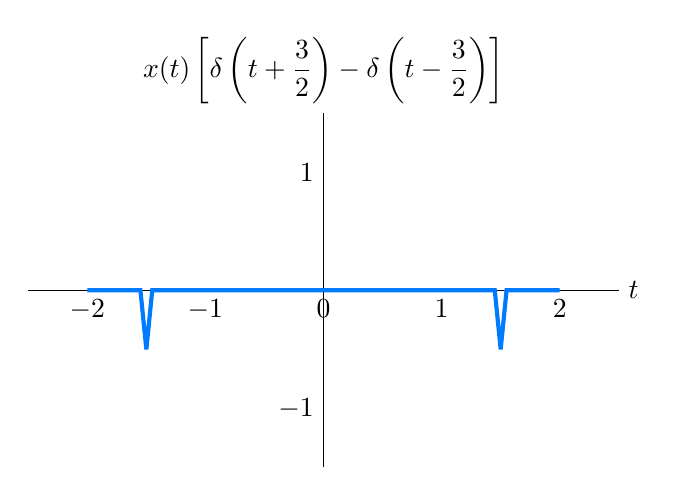
\begin{tikzpicture}[scale=1.5]
        \draw (-2.5,0) -- (2.5,0) node[right] {$t$};
        \draw (0,-1.5) -- (0,1.5) node[above] {$x(t)\left[ \delta\left( t+\dfrac{3}{2} \right) -\delta\left( t-\dfrac{3}{2} \right)  \right]$};
        \draw[lightblue, line width=1.5] (-2, 0) -- (-1.55, 0) -- (-1.5,-0.5) -- (-1.45, 0) -- (1.45, 0) -- (1.5,-0.5) -- (1.55, 0) -- (2,0);
        \foreach \x in {-2,...,2} {\node[below] at (\x,0) {$\x$};}
        \foreach \y in {-1, 1} {\node[left] at (0,\y) {$\y$};}
      \end{tikzpicture}
    \end{center}
    \end{enumerate}
  \item \lb{La figura 2 muestra la señal discreta $x[n]$. Represente cada una de las siguientes señales:}
    \begin{center}
      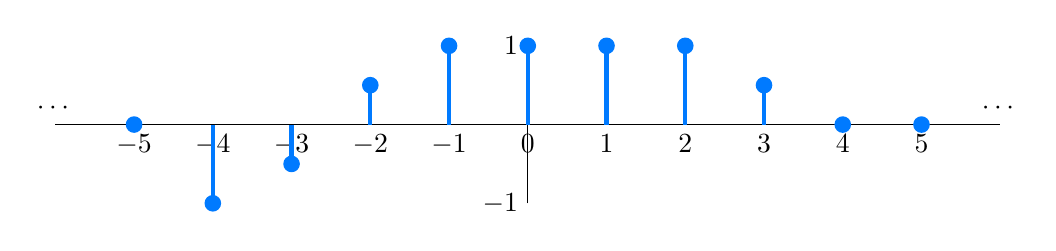
\begin{tikzpicture}
        \draw (-6,0) node[above] {$\cdots$} -- (6,0) node[above] {$\cdots$};
        \draw (0,-1) node[left] {$-1$} -- (0,1) node[left] {$1$};
        \foreach \x/\y in {-5/0,-4/-1,-3/-0.5,-2/0.5, -1/1, 0/1, 1/1, 2/1, 3/0.5, 4/0, 5/0} {
        \node[below] at (\x,0) {$\x$};
        \draw[lightblue, line width=1.5] (\x,0) -- (\x,\y);
        \fill[lightblue] (\x,\y) circle (3pt);
        }
      \end{tikzpicture}\\
      \lb{Figura 2} 
    \end{center}
    \begin{enumerate}[label=\color{red}\textbf{\alph*)}]
      \item \db{$x[n-4]$}
\begin{center} 
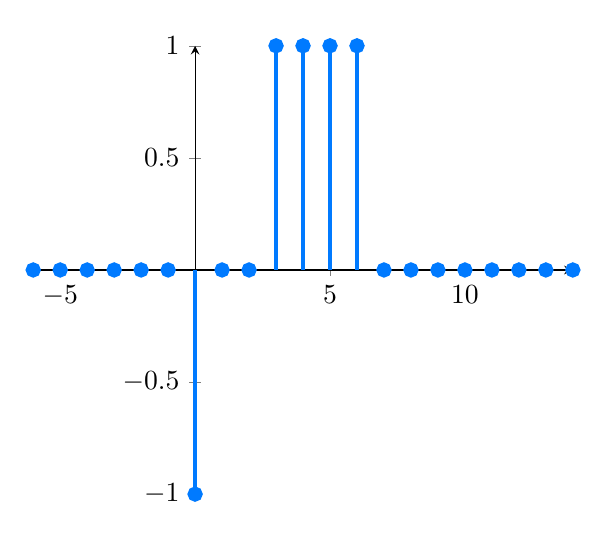
\begin{tikzpicture}
        \begin{axis}[
          axis lines = middle
        ]
        \addplot[lightblue, line width=1.5, ycomb, mark=*] coordinates {
(-6, 0) (-5, 0) (-4, 0) (-3, 0) (-2, 0) (-1, 0) (0, -1) (1, 0) (2, 0) (3, 1) (4, 1) (5, 1) (6, 1) (7, 0) (8, 0) (9, 0) (10, 0) (11, 0) (12, 0) (13, 0) (14, 0)
          };
        \end{axis}
      \end{tikzpicture}
\end{center}
      \item \db{$x[3-n]$} 
\begin{center}
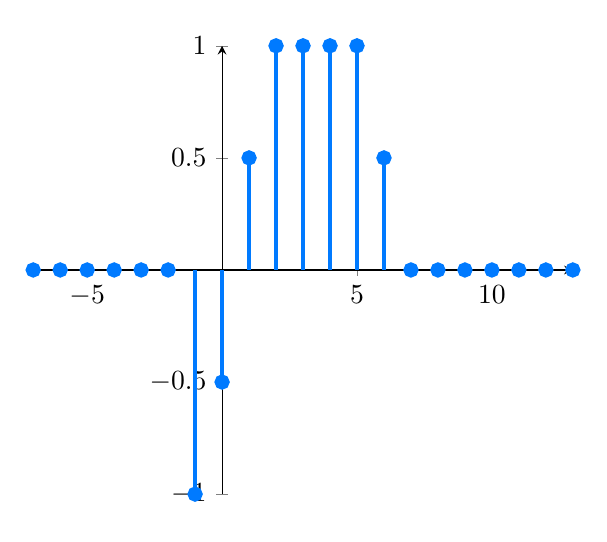
\begin{tikzpicture}
        \begin{axis}[
          axis lines = middle
        ]
        \addplot[lightblue, line width=1.5, ycomb, mark=*] coordinates {
(-7, 0.0) (-6, 0.0) (-5, 0.0) (-4, 0.0) (-3, 0.0) (-2, 0.0) (-1, -1.0) (0, -0.5) (1, 0.5) (2, 1.0) (3, 1.0) (4, 1.0) (5, 1.0) (6, 0.5) (7, 0.0) (8, 0.0) (9, 0.0) (10, 0.0) (11, 0.0) (12, 0.0) (13, 0.0)
          };
        \end{axis}
      \end{tikzpicture}
\end{center}
      \item \db{$x[3n]$} 
\begin{center}
\begin{tikzpicture}
        \begin{axis}[
          axis lines = middle
        ]
        \addplot[lightblue, line width=1.5, ycomb, mark=*] coordinates {
(-9, 0.0) (-6, 0.0) (-3, -0.5) (0, 1.0) (3, 0.5) (6, 0.0) (9, 0.0)
          };
        \end{axis}
      \end{tikzpicture}
\end{center}
      \item \db{$x[3n+1]$} 
\begin{center}
\begin{tikzpicture}
        \begin{axis}[
          axis lines = middle 
        ]
        \addplot[lightblue, line width=1.5, ycomb, mark=*] coordinates {
(-10, 0.0) (-7, 0.0) (-4, -0.5) (-1, 1.0) (2, 0.5) (5, 0.0) (8, 0.0)
          };
        \end{axis}
      \end{tikzpicture}
\end{center}
      \item \db{$x[n]u[3-n]$}
\begin{center}
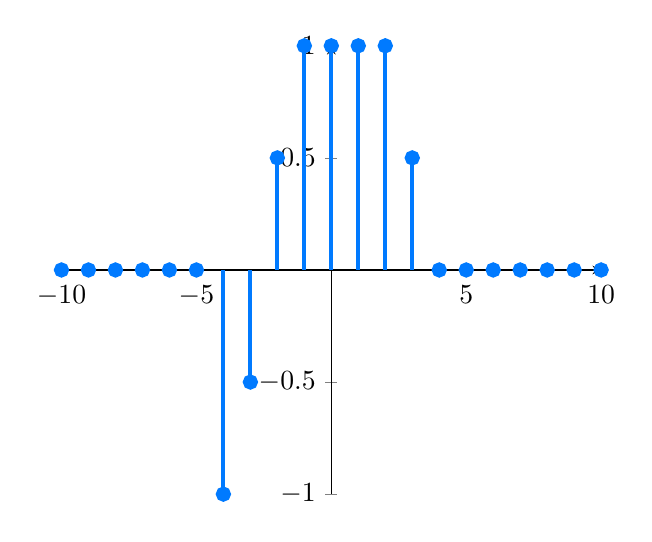
\begin{tikzpicture}
        \begin{axis}[
          axis lines = middle
        ]
        \addplot[lightblue, line width=1.5, ycomb, mark=*] coordinates {
(-10, 0.0) (-9, 0.0) (-8, 0.0) (-7, 0.0) (-6, 0.0) (-5, 0.0) (-4, -1.0) (-3, -0.5) (
-2, 0.5) (-1, 1.0) (0, 1.0) (1, 1.0) (2, 1.0) (3, 0.5) (4, 0.0) (5, 0.0) (6, 0.0) (7
, 0.0) (8, 0.0) (9, 0.0) (10, 0.0)
          };
        \end{axis}
      \end{tikzpicture}
\end{center} 
      \item \db{$x[n-3]\delta[n-2]$} 
\begin{center}
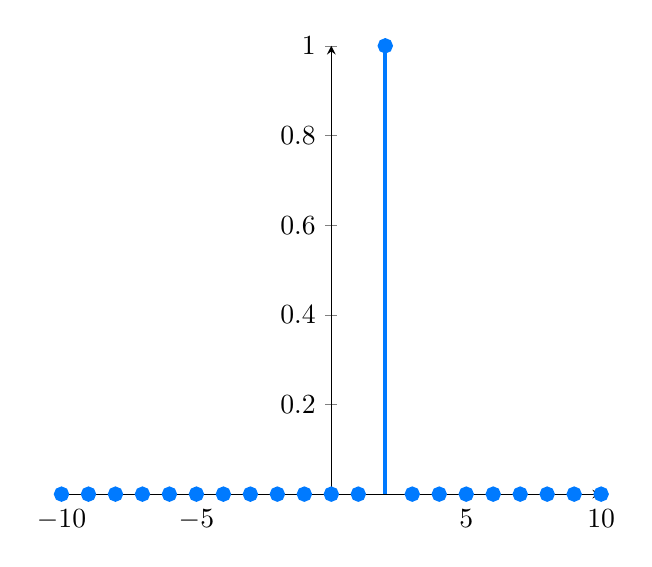
\begin{tikzpicture}
        \begin{axis}[
          axis lines = middle
        ]
        \addplot[lightblue, line width=1.5, ycomb, mark=*] coordinates {
(-10, 0) (-9, 0) (-8, 0) (-7, 0) (-6, 0) (-5, 0) (-4, 0) (-3, 0) (-2, 0) (-1, 0) (0,
 0) (1, 0) (2, 1) (3, 0) (4, 0) (5, 0) (6, 0) (7, 0) (8, 0) (9, 0) (10, 0)
          };
        \end{axis}
      \end{tikzpicture}
\end{center}
      \item \db{$\dfrac{1}{2}x[n]+\dfrac{1}{2}(-1)^nx[n]$}
\begin{center}
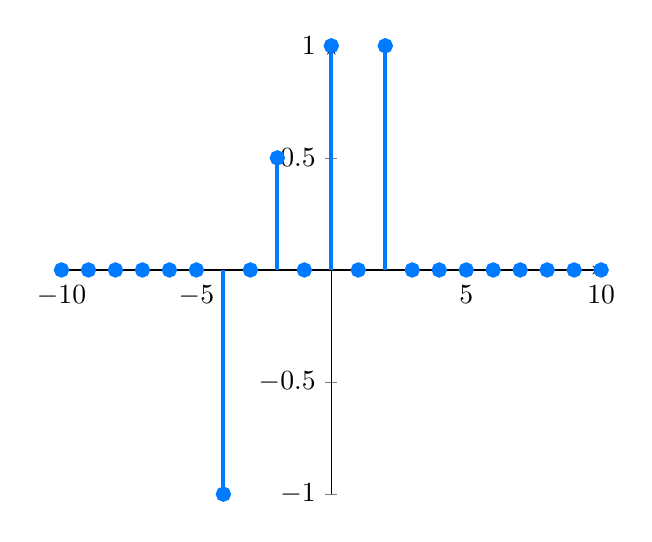
\begin{tikzpicture}
        \begin{axis}[
          axis lines = middle
        ]
        \addplot[lightblue, line width=1.5, ycomb, mark=*] coordinates {
(-10, 0.0) (-9, 0.0) (-8, 0.0) (-7, 0.0) (-6, 0.0) (-5, 0.0) (-4, -1.0) (-3, 0.0) (-
2, 0.5) (-1, 0.0) (0, 1.0) (1, 0.0) (2, 1.0) (3, 0.0) (4, 0.0) (5, 0.0) (6, 0.0) (7,
 0.0) (8, 0.0) (9, 0.0) (10, 0.0)
          };
        \end{axis}
      \end{tikzpicture}
\end{center} 
      \item \db{$x[(n-1)^2]$} 
\begin{center}
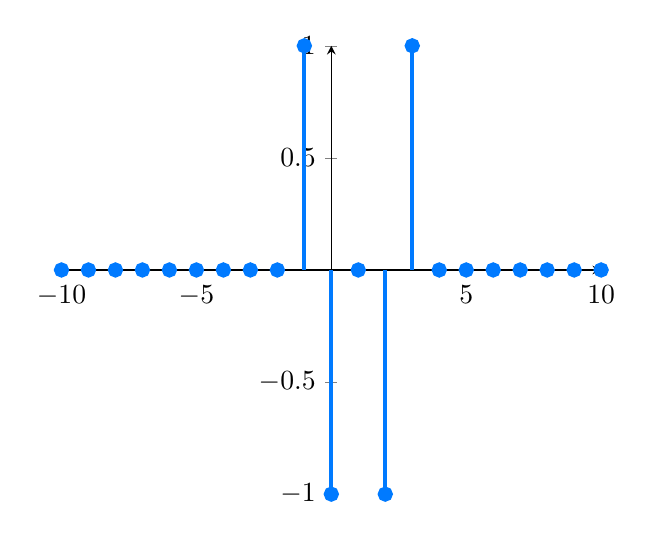
\begin{tikzpicture}
        \begin{axis}[
          axis lines = middle
        ]
        \addplot[lightblue, line width=1.5, ycomb, mark=*] coordinates {
(-10, 0.0) (-9, 0.0) (-8, 0.0) (-7, 0.0) (-6, 0.0) (-5, 0.0) (-4, 0.0) (-3, 0.0) (-2, 0.0) (-1, 1.0) (0, -1.0) (1, 0.0) (2, -1.0) (3, 1.0) (4, 0.0) (5, 0.0) (6, 0.0) (7, 0.0) (8, 0.0) (9, 0.0) (10, 0.0)
          };
        \end{axis}
      \end{tikzpicture}
\end{center}
    \end{enumerate}
  \item \lb{Determine si cada una de las siguientes señales continuas es periódica. En caso afirmativo obtenga su periodo fundamental.}
    \begin{enumerate}[label=\color{red}\textbf{\alph*)}]
      \item \db{$x(t)=3\cos\left(4t+\dfrac{\pi}{3}\right)$} 

          La señal es una función coseno, que es periódica si su frecuencia angular $\omega=4$ es finita. El periodo fundamental se calcula como: \[
          T_0=\dfrac{2\pi}{\omega}=\dfrac{2\pi}{4})\dfrac{\pi}{2}.
          \] 
          Por lo tanto, \textbf{la señal es periódica} con periodo fundamental $T_0=\dfrac{\pi}{2}$.
      \item \db{$x(t)=e^{j(\pi t-1)} $} 
          
          Esta señal es una exponencial compleja, que puede expresarse como: \[
          x(t)=e^{-j}\cdot e^{j\pi t}.  
          \] 
          El término $e^{-j} $ es una constante, y el término $e^{j\pi t} $ es periódico si su frecuencia angular $\omega=\pi$ es finita. El periodo fundamental se calcula como: \[
          t_0=\dfrac{2\pi}{\omega}=\dfrac{2\pi}{\pi})2.
          \] 
          Por lo tanto, \textbf{la señal es periódica} con periodo fundamental $T_0=2$.
      \item \db{$x(t)=\cos^2\left( 2t-\dfrac{\pi}{3} \right) $} 

          Utilizamos la identidad trigonométrica: \[
          \cos^2(\theta)=\dfrac{1+\cos(\theta)}{2}.
          \] 
          Sustituyendo $\theta=2t-\dfrac{\pi}{3}$, tenemos: \[
          x(t)=\dfrac{1}{2}+\dfrac{1}{2}\cos\left( 2\left( 2t-\dfrac{\pi}{3} \right)  \right) =\dfrac{1}{2}+\dfrac{1}{2}\cos\left( 4t-\dfrac{2\pi}{3} \right) .
          \] 
          El primer término $\left( \dfrac{1}{2} \right) $ es constante, y el segundo término es un conseno con frecuencia angular $\omega=4$. El periodo fundamental de este término es: \[
          T_0=\dfrac{2\pi}{\omega}=\dfrac{2\pi}{4}=\dfrac{\pi}{2}.
          \] 
          Por lo tanto, \textbf{la señal es periódica} con periodo fundamental $T_0=\dfrac{\pi}{2}$.
      \item \db{$x(t)=\mathrm{Par}\{\cos(4\pi t)u(t)\} $} 

          Aquí, $u(t)$ es la función escalón unitario, que es no nula solo para $t\ge 0$. La función $\mathrm{Par}\{\cdot \} $ denota la parte par de la señal, definida como: \[
          \mathrm{Par}\{x(t)\} =\dfrac{x(t)+x(-t)}{2}.
          \] 
          Susituyendo $x(t)=\cos(4\pi t)u(t)$, tenemos: \[
          \mathrm{Par}\{\cos(4\pi t)u(t)\} =\dfrac{\cos(4\pi t)u(t)+\cos(-4\pi t)u(-t)}{2}.
          \] 
          Para $t\ge 0,u(t)=1$ y $u(-t)=0$, mientras que  $t<0,u(t)=0$ y $u(-t)=1$. Esto implica que la señal no es continua en todo  $t$, y por lo tanto  \textbf{no es periódica}. 
      \item \db{$x(t)=\mathrm{Par}\{\sin(4\pi t)u(t)\} $} 

          Aquí, $u(t)$ es la función escalón unitario, que es no nula solo para $t\ge 0$. La función $\mathrm{Par}\{\cdot \} $ denota la parte par de la señal, definida como: \[
          \mathrm{Par}\{x(t)\} =\dfrac{x(t)+x(-t)}{2}.
          \] 
          Susituyendo $x(t)=\sin(4\pi t)u(t)$, tenemos: \[
          \mathrm{Par}\{\sin(4\pi t)u(t)\} =\dfrac{\sin(4\pi t)u(t)+\sin(-4\pi t)u(-t)}{2}.
          \] 
          Para $t\ge 0,u(t)=1$ y $u(-t)=0$, mientras que  $t<0,u(t)=0$ y $u(-t)=1$. Esto implica que la señal no es continua en todo  $t$, y por lo tanto  \textbf{no es periódica}. 

      \item \db{$x(t)=\sum_{n=-\infty}^{\infty} e^{-(2t-n)}u(2t-n) $} 

          Esta señal es una suma infinita de términos desplazados y modulados por la función escalón unitario $u(2t-n)$. Para analizar su periodicidad, debemos verificar si existe un $T>0$ tal que $x(t+T)=x(t)$.

          El término  $u(2t-n)$ es no nulo solo cuando  $2t-n\ge 0$, es decir, $t\ge \dfrac{n}{2}$. Esto significa que cada término de la suma está activo sólo en un intervalo específico. Debido a la dependencia de $n$ y la naturaleza de la suma, la señal \textbf{no es periódica}. 
    \end{enumerate}
\item \lb{Determine si cada una de las siguientes señales discretas es periódica. En caso afirmativo obtenga su periodo fundamental.}
    \begin{enumerate}[label=\color{red}\textbf{\alph*)}]
        \item \db{$x[n]=\sin\left( \dfrac{6\pi}{7}n+1 \right) $} 

            La frecuencia angular de la señal es $\omega=\dfrac{6\pi}{7}$. Para que la señal sea periódica, $\omega$ debe ser un múltiplo racional de $2\pi$, es decir, $\dfrac{\omega}{2\pi}=\dfrac{6}{7}$ debe ser racional. Esto es cierto, ya que $\dfrac{6}{7}$ es una fracción irreducible.

            El periodo fundamental $N$ se calcula como el denominador del cociente $\dfrac{\omega}{2\pi}$, es decir: \[
            N=7.
            \] Por lo tanto, \textbf{la señal es periódica} con periodo fundamental $N=7$.

        \item \db{$x[n]=\cos\left( \dfrac{n}{8}-\pi \right) $} 

            La frecuencia angular de la señal es $\omega=\dfrac{1}{8}$. Para que la señal sea periódica, $\dfrac{\omega}{2\pi}=\dfrac{1}{16\pi}$ debe ser racional. Sin embargo, $\dfrac{1}{16\pi}$ no es racional porque $\pi$ es irracional. Por lo tanto, \textbf{la señal no es periódica.} 
        \item \db{$\cos\left( \dfrac{\pi}{8}n^2 \right) $} 

            En este caso, la frecuencia angular depende de $n^2$, lo que significa que la señal no tiene una frecuencia angular constante. Esto implica que la señal no puede ser periódica, ya que no existe un $N$ tal que $x[n+N]=x[n]$ para todo $n$. Por lo tanto,  \textbf{la señal no es periódica}. 
        \item \db{$x[n]=\cos\left( \dfrac{\pi}{2}n \right) \cos\left( \dfrac{\pi}{4}n \right) $} 

            Utilizamos la identidad trigonométrica para el producto de cosenos: \[
            \cos(a)\cos(b)=\dfrac{1}{2}\left[ \cos(a-b)+\cos(a+b) \right] .
            \] 
            Sustituyendo $a=\dfrac{\pi}{2}$ y $b=\dfrac{\pi}{4}n$, tenemos: \[
                x[n]=\dfrac{1}{2}\left[ \cos\left( \dfrac{\pi}{2}n-\dfrac{\pi}{4}n \right) +\cos\left( \dfrac{\pi}{2}n+\dfrac{\pi}{4}n \right)  \right] =\dfrac{1}{2}\left[ \cos\left( \dfrac{\pi}{4}n \right) +\cos\left( \dfrac{3\pi}{4}n \right)  \right] .
            \] 
            La señal es la suma de dos cosenos con frecuencias angulares $\omega_1=\dfrac{\pi}{4}$ y $\omega_2=\dfrac{3\pi}{4}$. Para que la señal sea periódica, ambas frecuencias deben ser múltiplos racionales de $2\pi$, y el periodo fundamental será el mínimo común múltiplo (mcm) de sus periodos individuales.
            \begin{itemize}[label=\textbullet]
                \item Para $\omega_1=\dfrac{\pi}{4}$, el periodo $N_1=\dfrac{2\pi}{\omega_1}=8$.
                \item Para $\omega_2=\dfrac{3\pi}{4}$, el periodo $N_2=\dfrac{2\pi}{\omega_2}=\dfrac{8}{3}$, que no es entero.
            \end{itemize}
            Dado que $N_2$ no es entero, \textbf{la señal no es periódica.} 
            
        \item \db{$x[n]=2\cos\left( \dfrac{\pi}{4}n \right) +\sin\left( \dfrac{\pi}{8}n \right) -2\cos\left( \dfrac{\pi}{2}n +\dfrac{\pi}{6}\right) $} 

            La señal es una combinación lineal de tres términos con diferentes frecuencias angulares: 
            \begin{itemize}[label=\textbullet]
                \item $\omega_1=\dfrac{\pi}{4}$ 
                \item $\omega_2=\dfrac{\pi}{8}$ 
                \item $\omega_3=\dfrac{\pi}{2}$
            \end{itemize}
            Para que la señal sea periódica, todas las frecuencias deben ser múltiplos racionales de $2\pi$, y el periodo fundamental será el mcm de los periodos individuales.
            \begin{itemize}[label=\textbullet]
                \item Para $\omega_1=\dfrac{\pi}{4}$, el periodo es $N_1=\dfrac{2\pi}{\omega_1}=8$.
                \item Para $\omega_2=\dfrac{\pi}{8}$, el periodo es $N_2=\dfrac{2\pi}{\omega_2}=16$.
                \item Para $\omega_3=\dfrac{\pi}{2}$, el periodo es $N_3=\dfrac{2\pi}{\omega_3}=4$.
            \end{itemize}
            El mcm de $N_1=8,N_2=16$ y $N_3=4$ es $16$. Por lo tanto,  \textbf{la señal es periódica} con periodo fundamental $N=16$. 
    \end{enumerate}
\item \lb{Determine el módulo, así como la parte real e imaginaria de la señal \[
x(t)=te^{j_3\pi t}\prod\left( \dfrac{2t-4}{8} \right) -2\delta(2t+3) 
\]}

\begin{enumerate}[label=Paso \arabic*:]
    \item Descomposición de la señal

        La señal tiene dos términos:
        \begin{itemize}[label=\textbullet]
            \item $te^{j 3\pi t}\prod\left( \dfrac{2t-4}{8} \right)  $: Este término es una función ocnitnua que incluye un factor exponencia complejo, una función rectangular $\left( \prod \right) $ y un término lineal $t$.
            \item $-2\delta(2t+3)$: Este término es un impulso desplazado y escalado.
        \end{itemize}
        Analizaremos cada término por separado.
    \item Análisis del primer término $te^{j 3\pi t}\prod\left( \dfrac{2t-4}{8} \right)  $ 
        \begin{enumerate}[label=\alph*)]
            \item Parte exponencial $e^{j 3\pi t} $ 

                La exponencial compleja puede escribirse como: \[
                e^{j 3\pi t}=\cos(3\pi t)+j\sin(3\pi t). 
                \] 
                Por lo tanto, el término completo se convierte en: \[
                    te^{j 3\pi t}=t[\cos(3\pi t)+j\sin(3\pi t)] .
                \] 
            \item Función rectangular $\prod\left( \dfrac{2t-4}{8} \right) $

                La función rectangular $\prod(x)$ está definida como:  \[
                \prod(x)=\begin{cases}
                    1, & \text{si }|x|\le \dfrac{1}{2}\\
                    0, & \text{si }|x| > \dfrac{1}{2}
                \end{cases}
                \] 
                En este caso, el argumento de la función es $\dfrac{2t-4}{8}$, lo que implica que la función rectangular es no nula cuando: \[
                \left| \dfrac{2t-4}{8} \right| \le \dfrac{1}{2}.
                \] 
                Resolviendo la desigualdad: \[
                -\dfrac{1}{2}\le \dfrac{2t-4}{8}\le \dfrac{1}{2}\longrightarrow -4\le 2t-4\le 4\longrightarrow 0\le 2t\le 8\longrightarrow 0\le t\le 4.
                \] 
                Por lo tanto, la función rectangular $\prod\left( \dfrac{2t-4}{8} \right) $ es igual a 1 en el intervalo $t\in [0,4]$, y 0 fuera de este intervalo.
            \item Producto completo

                El primer término de la señal es: \[
               te^{j 3\pi t}\prod\left( \dfrac{2t-4}{8} \right) =\begin{cases}
                   t[\cos(3\pi t)+j\sin(3\pi t)], & \text{si }t\in [0,4]\\
                   0, & \text{si }t\notin [0,4]
               \end{cases}  
                \] 
        \end{enumerate}
    \item Análisis del segundo término $-2\delta(2t+3)$

        El término  $\delta(2t+3)$ es un impulso desplazado. La propiedad de escalamiento y desplazamiento del delta de Dirac nos dice que:  \[
        \delta(2t+3)=\dfrac{1}{2}\delta\left( t+\dfrac{3}{2} \right) .
        \] 
        Por lo tanto, el segundo término se convierte en: \[
        -2\delta(2t+3)=-2\cdot \dfrac{1}{2}\delta\left( t+\dfrac{3}{2} \right) =-\delta\left( t+\dfrac{3}{2} \right) .
        \] 
    \item Parte real, imaginaria y módulo de $x(t)$

        La señal completa es:  \[
        x(t)=\begin{cases}
            t[\cos(3\pi t)+j\sin(3\pi t)], & \text{si }t\in [0,4]\\
            \delta\left( t+\dfrac{3}{2} \right) , & \text{si }t=-\dfrac{3}{2}\\
            0, & \text{en otro caso}
        \end{cases}
        \] 
        \begin{enumerate}[label=\textbf{\alph*)}]
            \item \textbf{Parte real} 

                La parte real de $x(t)$ es:  \[
                \mathrm{Re}\{x(t)\} =\begin{cases}
                    t\cos(3\pi t), & \text{si }t\in [0,4]\\
                    -\delta\left( t+\dfrac{3}{2} \right) , & \text{si }t=-\dfrac{3}{2}\\
                    0, & \text{en otro caso}
                \end{cases}
                \] 
            \item \textbf{Parte imaginaria}

                La parte imaginaria de $x(t)$ es:  \[
                \mathrm{Im}\{x(t)\} =\begin{cases}
                    t\sin(3\pi t), & \text{si }t\in [0,4]\\
                    0, & \text{en otro caso}
                \end{cases}
                \] 
            \item \textbf{Módulo}

                El módulo de $x(t)$ es: \[
                |x(t)|=\begin{cases}
                    \sqrt{(t\cos(3\pi t))^2+(t\sin(3\pi t))^2}, & \text{si }t\in [0,4]\\
                    \left| \delta\left( t+\dfrac{3}{2} \right)  \right| , & \text{si }t=-\dfrac{3}{2}\\
                    0, & \text{en otro caso}
                \end{cases}
                \] 
                Simplificando el módulo en $t\in [0,4]$: \[
                |x(t)|=\sqrt{t^2\cos^2(3\pi t)+t^2\sin^2(3\pi t)}=\sqrt{t^2(\cos^2(3\pi t)+\sin^2(3\pi t))}=\sqrt{t^2}=|t|.   
                \] 
                Por lo tanto: \[
                |x(t)|=\begin{cases}
                    t, & \text{si }t\in [0,4]\\
                    \left| \delta\left( t+\dfrac{3}{2} \right)  \right| , & \text{si }t=-\dfrac{3}{2}\\
                    0, & \text{en otro caso}
                \end{cases}
                \] 
        \end{enumerate}
\end{enumerate}
\item \lb{Calcule la energía y la potencia de la señal mostrada en la figura 3. Indique si se encuentra definida en enegería o en potencia.}
\begin{center}
    \begin{tikzpicture}[>=latex,scale=0.7]
        \draw[->] (-10,0) -- (10,0) node[right] {$t$};
        \draw[->] (0,-2.5) -- (0,2.5) node[above] {$x(t)$};
        \foreach \x in {0,4,8} {\draw (\x,0.1) -- (\x,-0.1) node[below right] {$\x$};}
        \foreach \y in {-2,2} {\draw (0.1,\y) -- (-0.1,\y) node[left] {$\y$};}
            \draw[lightblue, line width=1.5] (-10,0) -- (0,0) -- (0,2) -- (4,2) -- (4,-2) -- (8,-2) -- (8,0) -- (9.5,0);
    \end{tikzpicture}\\
    \lb{Figura 3} 
\end{center}
La señal $x(t)$ es una señal a trozos definida como: \[
x(t)=\begin{cases}
    2, & 0\le t<4\\
    -2, & 4\le t<8\\
    0, & \text{en otro caso}
\end{cases}
\] 
La energía de una señal $x(t)$ se define como:  \[
E=\int_{-\infty}^{\infty} |x(t)|^2\dt .
\] 
Dado que $x(t)$ es no nula solo en el intervalo $[0,8]$, la integral se reduce a:  \[
E=\int_{0}^{4} |2|^2\dt+\int_{4}^{8} |-2|^2\dt.  
\] 
Calculamos cada término:
\begin{itemize}[label=\textbullet]
    \item Para $0\le t<4,x(t)=2$, entonces: \[
            \int_{0}^{4} |2|^2\dt=\int_{0}^{4} 4\dt=4 \int_{0}^{4} 1\dt=4[t]_0^4=4\cdot (4-0)=16.   
    \] 
\item Para $4\le t<8, x(t)=-2$, entonces: \[
        \int_{4}^{8} |-2|^2\dt=\int_{4}^{8} 4\dt=4 \int_{4}^{8} 1\dt=4[t]_4^8=4\cdot (8-4)=16   
\] 
\end{itemize}
Sumando ambos términos: \[
E=16+16=32.
\] 
Por lo tanto, la \textbf{energía de la señal} es: \[
E=32.
\] 
La potencia de una señal $x(t)$ se define como:  \[
P=\lim_{T \to \infty} \dfrac{1}{2T}\int_{-T}^{T} |x(t)|^2\dt=\lim_{T \to \infty} \dfrac{E}{2T}=\dfrac{32}{\infty}=0. 
\] 
Por lo tanto, la señal está \textbf{definida en energía}. 
\item \lb{Represente detalladamente las señales $x_1(t)$ y $x(t)$, definidas como \[
\begin{array}{c}
    x_1(t)=2\prod\left( \dfrac{t}{4} \right) +(6-2t)\left[ \prod\left( \dfrac{t-2.5}{1} \right) -\prod\left( \dfrac{t-3.5}{1} \right)  \right] \\
    x(t)=\sum_{n=-\infty}^{\infty} x_1(t-6n)
\end{array}
\] } 
\begin{center}
\includegraphics[width=0.45\textwidth]{"20_1"}\qquad
\includegraphics[width=0.45\textwidth]{"20_2"}
\end{center}
\item \lb{Represente detalladamente las señales $x(t)$ y  $h(t)$ dadas por  \[
            \begin{array}{c}
            x(t)=t\prod\left( \dfrac{2t}{4} \right) +t[u(t-1)-u(3t-9)]\\
            h(t)=2\prod\left( \dfrac{t-1}{4} \right) +\delta(t+4)
            \end{array}
\] } 
\begin{center}
\includegraphics[width=0.45\textwidth]{"21_1"}\qquad
\includegraphics[width=0.45\textwidth]{"21_2"}
\end{center}
\item \lb{Calcule la energía y la potencia de la señal $x(t)$ del ejercicio 21, indicando si se trata de una señal definida en energía  o en potencia.}

    La señal $x(t)$ está compuesta por dos términos:
    \begin{itemize}[label=\textbullet]
        \item \textbf{Primer término:} $t\prod\left( \dfrac{2t}{4} \right) $, que incluye una función rectangular $\prod(x)$. La función rectangular $\prod(x)$ está definida como:  \[
        \prod(x)=\begin{cases}
            1, & \text{si }|x|\le \dfrac{1}{2}\\
            0, & \text{si }|x| > \dfrac{1}{2}
        \end{cases}
        \]  
        En este caso, el argumento es $\dfrac{2t}{4}=\dfrac{t}{2}$, por lo que la función de ventana es no nula solo cuando: \[
        \left| \dfrac{t}{2} \right| \le \dfrac{1}{2}\longrightarrow -1\le t\le 1.
        \] 
        Por lo tanto, el primer término es no nulo únicamente en el intervalo $t\in [-1,1]$, y en este intervalo vale $t$.
    \item  \textbf{Segundo término:} $t[u(t-1)-u(3t-9)]$, que incluye funciones escalón unitario $u(t)$. Analicemos los intervalos donde este término es no nulo:
        \begin{itemize}[label=\textbullet]
            \item $u(t-1)$ es no nulo para  $t\ge 1$.
            \item $u(3t-9)$ es no nulo para  $t\ge 3$.
        \end{itemize}
        Por lo tanto, $u(t-1)-u(3t-9)$ es no nulo en el intervalo  $1\le t<3$, y en este intervalo vale 1. Entonces, el segundo término es: \[
            t[u(t-1)-u(3t-9)]=\begin{cases}
                t, & \text{si }1\le t<3\\
                0, & \text{en otro caso}
            \end{cases}
        \] 
    \end{itemize}
    Combinando ambos términos, la señal $x(t)$ se puede escribir como: \[
    x(t)=\begin{cases}
        t, & \text{si }-1\le t\le 1\\
        t, & \text{si }1\le t<3\\
        0, & \text{en otro caso}
    \end{cases}=\begin{cases}
        t, & \text{si }-1\le t<3\\
        0, & \text{en otro caso}
    \end{cases}
    \]
    La energía de una señal $x(t)$ se define como: \[
    E=\int_{-\infty}^{\infty} |x(t)|^2\dt. 
    \] 
    Dado que $x(t)$ es no nula solo en el intervalo  $t\in [-1,3]$, la integral se reduce a: \[
    E=\int_{-1}^{3} |t|^2\dt=\int_{-1}^{3} t^2\dt=\left[ \dfrac{t^3}{3} \right] _{-1}^3=\dfrac{3^3}{3}-\dfrac{(-1)^3}{3}=\dfrac{27}{3}-\dfrac{-1}{3}=9+\dfrac{1}{3}=\dfrac{28}{3}.  
    \] 
    Por lo tanto, la \textbf{energía de la señal} es: \[
    E=\dfrac{28}{3}.
    \] 
    La potencia de una señal $x(t)$ se define como: \[
    P=\lim_{T \to \infty} \dfrac{1}{2T}\int_{-T}^{T} |x(t)|^2\dt=\lim_{T \to \infty} \dfrac{E}{2T}=\dfrac{\frac{28}{3} }{\infty}=0. 
    \] 
    Por lo tanto, la señal está \textbf{definida en energía}. 
\item \lb{Represente detalladamente las señales \[
\begin{array}{c}
    x[n]=e^{j\frac{\pi}{4} n} u[n]\\
    h[n]=\cos\left( \dfrac{\pi}{4}n \right) \prod\left( \dfrac{n-2}{11} \right) 
\end{array}
\] } 
\item \lb{Calcule la energía y la potncia de la señal $x[n]$ del ejercicio 23, indicando si se trata de una señal definida en energía o en potencia.}
\item \lb{Indique si la señal $x[n]$ del ejercicio 23 y la señal  $z[n]=x[n]+x^*[-n]$ son periódicas y, en su caso, obtenga el valor de los correspondientes periodos.}
\item \lb{Considere la señal continua no periódica mostrada en la figura 4 y represente su partes par e impar.}
    \begin{center}
        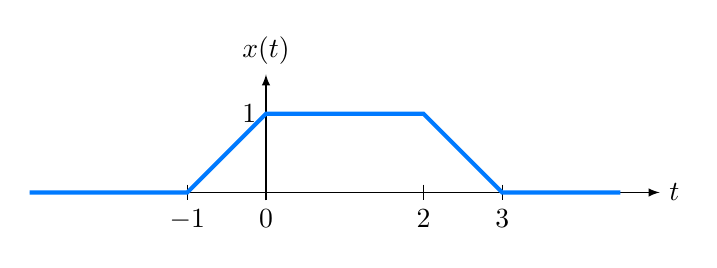
\begin{tikzpicture}
            \draw[-latex] (-3,0) -- (5,0) node[right] {$t$};
            \draw[-latex] (0,-0.1) -- (0,1.5) node[above] {$x(t)$};
            \foreach \x in {-1,0,2,3} {\draw (\x,0.1) -- (\x,-0.1) node[below] {$\x$};}
                \node[left] at (0,1) {$1$};
                \draw[lightblue, line width=1.5] (-3,0) -- (-1,0) -- (0,1) -- (2,1) -- (3,0) -- (4.5,0);
        \end{tikzpicture}\\
        \lb{Figura 4} 
    \end{center}
\item \lb{Calcule la energía y la potencia de la señal de la figura 4, indicando si se trata de una señal definida en energía o en potencia.}

\item \lb{Represente detalladamente las siguientes señales: \[
\begin{array}{c}
    x[n]=\left( \dfrac{1}{2} \right) ^{2n}(u[n+3]-u[n+4]u[-n-5])\\
    h[n]=3^nu[-n-1]+3^{-n-1}u[n]
\end{array}
\] } 
\item \lb{Calcule la energía y la potencia de la señal $x[n]$ del ejercicio 28, indicando si se trata de una señal definida en energía o en potencia.}
\item \lb{Calcule la energía y la potencia de la señal de la figura 5, indicando si está definida en energía o en potencia.}
    \begin{center}
        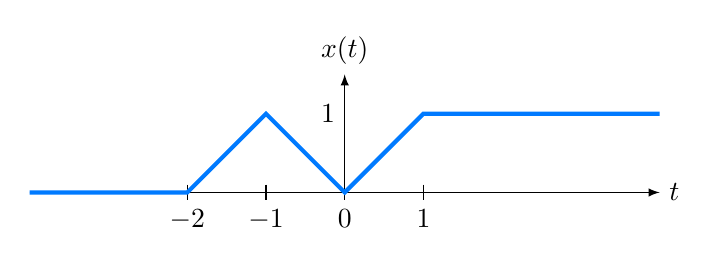
\begin{tikzpicture}
            \draw[-latex] (-4,0) -- (4,0) node[right] {$t$};
            \draw[-latex] (0,0) -- (0,1.5) node[above] {$x(t)$};
            \foreach \x in {-2,-1,0,1} {\draw (\x,0.1) -- (\x,-0.1) node[below] {$\x$};}
                \node[left] at (0,1) {$1$};
                \draw[lightblue, line width=1.5] (-4,0) -- (-2,0) -- (-1,1) -- (0,0) -- (1,1) -- (4,1);
        \end{tikzpicture}
    \\
    \lb{Figura 5} 
    \end{center}
\item \lb{Represente detalladamente las señales \[
\begin{array}{c}
    x(t)=-\left( \dfrac{t}{2}+1 \right) \prod\left( \dfrac{t}{4} \right) \\
h(t)=1-u(t-1)u(t-3)-u(1-t)
\end{array}
\] } 
\item \lb{Calcule la energía y la potencia de la señal $x(t)$ del ejercicio 31, indicando si se trata de una señal definida en energía o en potencia.}
\item \lb{Represente detalladamente la señal \[
x(t)=\dfrac{1+\mathrm{sign}(\sin(t))}{2}\sin(t)
\] } 
\item \lb{Represente detalladamente las señales \[
x(t)=e^{-(2+j_3)t}u(t+3)\\
h(t)=\prod\left( \dfrac{t-1.5}{5} \right) -5\delta(t-5)
\] } 
\item \lb{Calcule la energía y la potencia de la señal $x(t)$ del ejercicio 34, indicando si se trata de una señal definida en energía o en potencia.}
\item \lb{Calcule la energía y la potencia de la señal $x(t)$, indicando si se trata de una señal definida en energía o en potencia.  \[
x(t)=\bigwedge\left( \dfrac{t}{b} \right) 
\] } 
\item \lb{Considere un sistema discreto cuya señal de entrada es $x[n]$ y la sñela de salida es  $y[n]$. La relación entre la entrada y la salida viene dada por  \[
            y[n]=x[n]x[n-2]
\] } 
\begin{enumerate}[label=\color{red}\textbf{\alph*)}]
    \item \db{¿Tiene memoria el sistema?} 

        Un sistema tiene memoria si su salida en un tiempo $n$ depende de valores pasados o futuros de la entrada.
         \begin{itemize}[label=\textbullet]
             \item La salida $y[n]$ se define en términos de  $x[n]$ y  $x[n-2]$.
             \item Como depende del valor presente  $x[n]$ y de un valor pasado  $x[n-2]$, el sistema tiene memoria.
        \end{itemize}
    \item \db{Determine la señal de salida del sistema cuando la entrada es $A\delta[n]$, siendo  $A$ una constante real o compleja.}

        Sustituyendo $A\delta[n]$ en la ecuación del sistema:  \[
            y[n]=x[n]x[n-2]=A\delta[n]\cdot A\delta[n-2].
        \] 
        Dado que $\delta[n]$ solo es distinto de cero cuando  $n=0$ y  $\delta[n-2]$ solo es distinto de cero cuando  $n=2$, su producto será diferente de cero si ambos índices coinciden, lo cual nunca ocurre.

        Por lo tanto:  \[
            y[n]=0, \forall n.
        \] 
    \item \db{¿Es invertible el sistema?} 
        Un sistema es invertible si podemos recuperar la entrada $x[n]$ a partir de la salida  $y[n]$.
         \begin{itemize}[label=\textbullet]
             \item De la ecuación $y[n]=x[n]x[n-2]$, observamos que hay dos valores de  $x[n]$ que intervienen en la salida.
             \item Si  $x[n]=0$ o  $x[n-2]=0$, entonces  $y[n]=0$, lo que significa que no podemos distinguir entre diferentes posibles entradas que produzcan la misma salida.
             \item Por lo tanto, el sistema no es invertible.
        \end{itemize}
\end{enumerate}
\item \lb{Considere un sistema continuo cuya señal de entrada es $x(t)$ y de salida  $y(t)$ relacionadas por  \[
y(t)=x(\sin(t))
\] } 
\begin{enumerate}[label=\color{red}\textbf{\alph*)}]
    \item \db{¿Es causal el sistema?}

        Un sistema es causal si la salida $y(t)$ en cualquier instante  $t$ depende únicamente de valores presentes o pasados de la entrada  $x(t)$, es decir, no puede depender de valores futuros de  $x(t)$.
         \begin{itemize}[label=\textbullet]
            \item  En este caso, la salida $y(t)=x(\sin(t))$ evalúa la entrada en $\sin(t)$, que no siempre es menor o igual a $t$.
            \item Como  $\sin(t)$ oscila en el intervalo $[-1,1]$, la salida en  $t$ depende de valores de la entrada en tiempos futuros y pasados.
        \end{itemize}
        Por lo tanto, el sistema no es causal.
    \item \db{¿Es lineal?} 

        Un sistema es lineal si cumple las propiedades de superposición y homogeneidad.
        \begin{enumerate}[label=\arabic*)]
            \item Superposición: Si $x_1(t)\to y_1(t)$ y $x_2(t)\to y_2(t)$, entonces: \[
            x_1(t)+x_2(t)\to y_1(t)+y_2(t).
            \] 
        \item Homogeneidad: Si $x(t)\to y(t)$, entonces: \[
        \alpha x(t)\to \alpha y(t)
        \] 
        \end{enumerate}
        Probemos si el sistema cumple estras propiedades:
        \begin{itemize}[label=\textbullet]
            \item Si tenemos dos entradas $x_1(t)$ y $x_2(t)$, entonces las salidas son: \[
            y_1(t)=x_1(\sin(t)),\: y_2(t)=x_2(\sin(t))
            \] 
        \item Si aplicamos la entrada combinada $x_1(t)+x_2(t)$, salida es: \[
        y(t)=(x_1+x_2)(\sin(t))=x_1(\sin(t))+x_2(\sin(t))=y_1(t)+y_2(t).
        \] 
        \end{itemize}
        La propiedad de superposición se cumple.

        Si aplicamos una constante $\alpha$, tenemos: \[
        y(t)=(\alpha x)(\sin(t))=\alpha x(\sin(t))=\alpha y(t).
        \] 
        Como se cumple la propiedad de homogeneidad, el sistema es lineal.

\end{enumerate}
\item \lb{Para cada una de las siguientes relaciones entrada-salida determine si el sistema correspondiente es lineal, invariante en el tiempo o ambos.}
    \begin{enumerate}[label=\color{red}\textbf{\alph*)}]
        \item \db{$y(t)=t^2x(t-1)$} 

            Para ser lineal, el sistema debe cumplir superposición y homogeneidad.

            Si la entrada es $x_1(t)$ con salida $y_1(t)$, y $x_2(t)$ con salida $y_2(t)$, entonces para la entrada combinada $x_1(t)+x_2(t)$, la salida debería ser: \[
            y(t)=t^2(x_1(t-1)+x_2(t-1))=t^2x_1(t-1)+t^2x_2(t-1)=y_1(t)+y_2(t)
            \] 
            Cumple superposición.

            Para homogeneidad: \[
            y(t)=t^2(\alpha x(t-1))=\alpha t^2x(t-1)=\alpha y(t).
            \] 
            Es lineal.

            Si desplazamos la entrada $x(t)\to x(t-t_0)$, la salida se convierte en: \[
            y'(t)=t^2x(t-1-t_0)
            \] pero la salida original desplazada es: \[
            y(t-t_0)=(t-t_0)^2x(t-t_0-1).
            \] 
            Como $(t-t_0)^2\neq t^2$, el sistema no es invariante en el tiempo.
        \item  \db{$y[n]=x^2[n-2]$} 

            Dado que la ecuación contiene $x[n]$ al cuadrado, no cumple la propiedad de superposición:  \[
                (x_1+x_2)^2\neq x_1^2+x_2^2.
            \] 
            Por lo tanto, no es lineal.

            Si desplazamos la entrada $x[n]\to x[n-k]$, la salida se convierte en: \[
                y'[n]=x^2[n-k-2]
            \] y la salida original desplazada es: \[
            y[n-k]=x^2[n-k-2]
            \] 
            Como ambas expresiones son iguales, es invariante en el tiempo.
        \item \db{$y[n]=x[n+1]-x[n-1]$} 

            Aplicamos superposición: \[
            \begin{aligned}
                y[n]&= (x_1+x_2)[n+1]-(x_1+x_2)[n-1] \\
                    &= x_1[n+1]+x_2[n+1]-x_1[n-1]-x_2[n-1] \\
                    &= (x_1[n+1]-x_1[n-1])+(x_2[n+1]-x_2[n-1]) \\
                    &= y_1[n]+y_2[n] \\
            \end{aligned}
            \] 
            Cumple superposición.

            Para homogeneidad: \[
                y[n]=\alpha x[n+1]-\alpha x[n-1]=\alpha y[n]
            \] 
            Es lineal.

            Si desplazamos la entrada $x[n]\to x[n-k]$, la salida se convierte en: \[
           \begin{aligned}
               y'[n]&= x[n+1-k]-x[n-1-k] \\
                    &= x[(n-k)+1]-x[(n-k)-1] \\
                    &= y[n-k] \\
           \end{aligned} 
            \] 
            Como la forma de la salida se mantiene tras el desplazamiento, es invariante en el tiempo.
        \item \db{$y(t)=\mathrm{Impar}\{x(t)\} $} 

            Recordemos que la parte impar de una señal se define como: \[
            \mathrm{Impar}\{x(t)\} =\dfrac{x(t)-x(-t)}{2}
            \] 
            Si tomamos dos entradas $x_1(t)$ y $x_2(t)$, aplicamos superposición: \[
           \begin{aligned}
               \mathrm{Impar}\{x_1(t)+x_2(t)\}&= \dfrac{x_1(t)+x_2(t)-x_1(-t)-x_2(-t)}{2} \\
               &= \dfrac{x_1(t)-x_1(-t)}{2} +\dfrac{x_2(t)-x_2(-t)}{2}\\
               &= \mathrm{Impar}\{x_1(t)\} +\mathrm{Impar}\{x_2(t)\}  \\
           \end{aligned} 
            \] 
            Cumple superposición.

            Para homogeneidad: \[
            \mathrm{Impar}\{\alpha x(t)\} =\dfrac{\alpha x(t)-\alpha x(-t)}{2}=\alpha\mathrm{Impar}\{x(t)\} 
            \] 
            Es lineal.

            Si desplazamos la entrada $x(t)\to x(t-t_0)$, la salida se convierte en \[
            y'(t)=\dfrac{x(t-t_0)-x(t-t_0)}{2}
            \] 
            Mientras que la señal original desplazada es: \[
            y(t-t_0)=\dfrac{x(t-t_0)-x(-t+t_0)}{2}.
            \] 
            Como las expresiones no son iguales, no es invariante en el tiempo.
    \end{enumerate}
\item \lb{Determine si cada uno de los siguientes sistemas es invertible. En caso afirmativo, construya el sistema inverso y, en caso negativo, encuentre dos señales de entrada al sistema que generen la misma señal de salida.}
    \begin{enumerate}[label=\color{red}\textbf{\alph*)}]
        \item \db{$y(t)=x(t-4)$} 
            \begin{itemize}[label=\textbullet]
                \item Invertible: Si
                \item Sistema inverso: $x(t)=y(t+4)$
            \end{itemize}
        \item \db{$y(t)=\cos(x(t))$} 
            \begin{itemize}[label=\textbullet]
                \item Invertible: No
                \item Razón: La función coseno no es inyectiva, ya que diferentes valores de $x(t)$ pueden producir el mismo  $y(t)$. Por ejemplo: 
                    \begin{center}
                        $x(t)=0$ y  $x(t)=2\pi$ generan $y(t)=1$.
                    \end{center}
            \end{itemize}
        \item \db{$y[n]=nx[n]$} 
            \begin{itemize}[label=\textbullet]
                \item Invertible: Si, para $n\neq 0$.
                \item Sistema inverso: $x[n]=\dfrac{1}{n}y[n]$ para $n\neq 0$.
            \end{itemize}
        \item \db{$y(t)=\int_{-\infty}^{t} x(\tau)\mathrm{d}\tau $} 
            \begin{itemize}[label=\textbullet]
                \item Invertible: Si
                \item Sistema inverso: $x(t)=\dfrac{\mathrm{d}}{\dt}y(t)$
            \end{itemize}
        \item \db{$y[n]=\begin{cases}
                    x[n-1], & n\ge 1\\
                    0, & n=0\\
                    x[n], & n\le -1
        \end{cases}$} 
    \item \db{$y[n]=x[n]x[n-1]$} 
    \item \db{$y[n]=x[1-n]$} 
        \item \db{$y(t)=\int_{-\infty}^{t} e^{-(t-\tau)}\mathrm{d}\tau  $} 
        \item \db{$y[n]=\sum_{k=-\infty}^{\infty} \left( \dfrac{1}{2} \right) ^{n-k}x[k]$} 
        \item \db{$y(t)=\dfrac{\mathrm{d}x(t)}{\dt}$} 
        \item \db{$y[n]=\begin{cases}
                    x[n+1], & n\ge 0\\
                    x[n], & n\le -1
        \end{cases}$} 
        \item \db{$y(t)=x(2t)$} 
        \item \db{$y[n]=x[2n]$} 
        \item \db{$y[n]=\begin{cases}
                    x\left[ \dfrac{n}{2} \right] , & \text{$n$ par}\\
                    0, & \text{$n$ impar}
        \end{cases}$} 
    \end{enumerate}
\item \lb{En este ejercicio se ilustra una de las consecuencias más importantes de las propiedades de linealidad e invarianza temporal. En concreto, cuando se conoce la respuesta de un sistema lineal e invariante en el tiempo (linear time-invariant systema, LTI) a una entrada determinada o la respuesta a varias entradas, se puede calcular la respuesta del sistema a otras señales de entrada.}
    \begin{center}
        \includegraphics[width=0.7\textwidth]{"41"}\\
        \lb{Figura 6} 
    \end{center}
    \begin{enumerate}[label=\color{red}\textbf{\alph*)}]
        \item \db{Considere un sistema LTI cuya respuesta a la señal $x_1(t)$ de la Figura 6(a) es la señal $y_1(t)$ mostrada en la Figura 6(b). Determine y represente la respuesta del sistema a la entrada $x_2(t)$ de la Figura 6(c).}

            Podemos expresar $x_2(t)$ en función de $x_1(t)$: \[
            x_2(t)=x_1(t)-x_1(t-2)
            \] 
            Al ser LTI podemos expresar su salida como: \[
            y_2(t)=y_1(t)-y_1(t-2)
            \] 
            \begin{center}
            \begin{tikzpicture}[baseline=(current bounding box.center)]
                \draw[-latex] (-0.5,0) -- (4.5,0) node[right] {$t$};
                \draw[-latex] (0,-2.5) -- (0,2.5) node[above] {$x_2(t)$};
                \foreach \y in {-2,-1,1,2} {\draw (0.1,\y) -- (-0.1,\y) node[left] {$\y$};}
                    \foreach \x in {0,1,...,4} {\draw (\x,0.1) -- (\x,-0.1) node[below] {$\x$};}
                        \draw[lightblue, line width=1.5] (0,0) -- (0,1) -- (2,1) -- (2,-1) -- (4,-1) -- (4,0);
            \end{tikzpicture}\qquad
            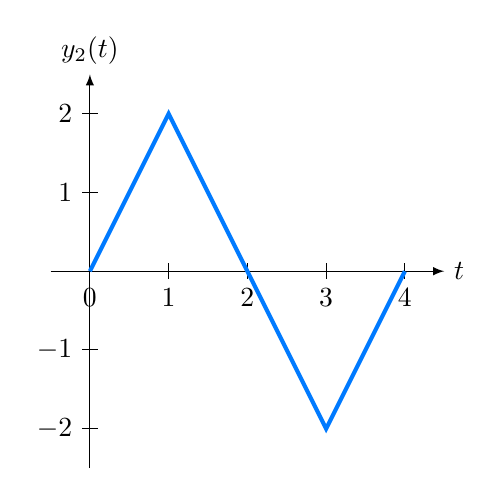
\begin{tikzpicture}[baseline=(current bounding box.center)]
                \draw[-latex] (-0.5,0) -- (4.5,0) node[right] {$t$};
                \draw[-latex] (0,-2.5) -- (0,2.5) node[above] {$y_2(t)$};
                \foreach \y in {-2,-1,1,2} {\draw (0.1,\y) -- (-0.1,\y) node[left] {$\y$};}
                    \foreach \x in {0,1,...,4} {\draw (\x,0.1) -- (\x,-0.1) node[below] {$\x$};}
                        \draw[lightblue, line width=1.5] (0,0) -- (1,2) -- (3,-2) -- (4,0);
            \end{tikzpicture}
        \end{center}
        \item \db{Determine y represente la respuesta del sistema considerado en el apartado anterior a la señal de entrada $x_3(t)$ mostrada en la Figura 6(d).} 

            Podemos expresar $x_3(t)$ en función de $x_1(t)$: \[
            x_3(t)=x_1(t+1)+x_1(t)
            \] 
            Al ser LTI, podemos expresar su salida como: \[
            y_3(t)=y_1(t+1)+y_1(t)
            \] 
            \begin{center}
            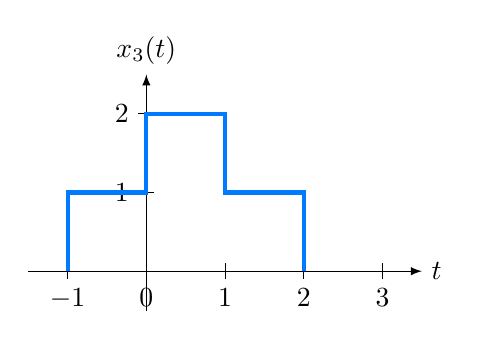
\begin{tikzpicture}[baseline=(current bounding box.center)]
                \draw[-latex] (-1.5,0) -- (3.5,0) node[right] {$t$};
                \draw[-latex] (0,-0.5) -- (0,2.5) node[above] {$x_3(t)$};
                \foreach \y in {1,2} {\draw (0.1,\y) -- (-0.1,\y) node[left] {$\y$};}
                    \foreach \x in {-1,0,1,...,3} {\draw (\x,0.1) -- (\x,-0.1) node[below] {$\x$};}
                        \draw[lightblue, line width=1.5] (-1,0) -- (-1,1) -- (0,1) -- (0,2) -- (1,2) -- (1,1) -- (2,1) -- (2,0);
            \end{tikzpicture}\qquad
            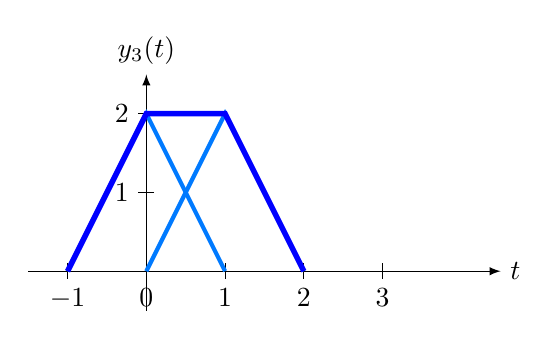
\begin{tikzpicture}[baseline=(current bounding box.center)]
                \draw[-latex] (-1.5,0) -- (4.5,0) node[right] {$t$};
                \draw[-latex] (0,-0.5) -- (0,2.5) node[above] {$y_3(t)$};
                \foreach \y in {1,2} {\draw (0.1,\y) -- (-0.1,\y) node[left] {$\y$};}
                    \foreach \x in {-1,0,1,...,3} {\draw (\x,0.1) -- (\x,-0.1) node[below] {$\x$};}
                        \draw[lightblue, line width=1.5] (-1,0) -- (0,2) -- (1,0);
                        \draw[lightblue, line width=1.5] (0,0) -- (1,2) -- (2,0);
                        \draw[blue, line width=2] (-1,0) -- (0,2) -- (1,2) -- (2,0);

            \end{tikzpicture}
                
            \end{center}
    \end{enumerate}
\item \lb{La salida de un sistema viene dada por $y[n]=x[2+n]x[2-n]$. Indique razonadamente si el sistema cumple las propiedades de memoria, causalidad, estabilidad, invarianza en el tiempo y linealidad.}
\item \lb{Considere la señal $x[n]=\bigwedge\left( \dfrac{n}{3} \right) +\bigwedge\left( \dfrac{n-3}{3} \right) $. Obtenga y represente las partes par e impar de dicha señal. Asimismo, calcule la energía y la potencia de $x[n]$, indicando si se trata de una señal definida en energía o en potencia.}
\item \lb{Calcule la energía y la potencia de $x[n]$, indicando si se trata de una señal definida en energía o en potencia.  \[
            x[n]=(u[n+6]-u[n-7]+\delta[-n+10])u[-n+10]
\] } 
\item \lb{Calcule la energía y la potencia de $x(t)$, indicando si se trata de una señal definida en energía o en potencia.  \[
x(t)=(t-2)u(t-1)u(4-t)\prod\left( \dfrac{t}{10} \right) 
\] } 
\item \lb{Determine si cada uno de los siguientes sistemas verifica las propiedades de memoria, causalidad, estabilidad, invarianza y linealidad.}
    \begin{enumerate}[label=\color{red}\textbf{\alph*)}]
        \item \db{$y(t)=e^{x(t)} $} 
        \item \db{$y[n]=x[n]x[n-1]$} 
        \item \db{$y(t)=\dfrac{\mathrm{d}x(t)}{\dt}$} 
        \item \db{$y[n]=x[-n]$} 
        \item \db{$y(t)=\sin(6t)x(t)$} 
        \item \db{$y[n]=\sum_{k=-2}^{n+4} $} 
        \item \db{$y[n]=nx[n]$} 
        \item \db{$y[n]=x[2n]$} 
    \end{enumerate}
\end{enumerate}
\end{document}
